\documentclass[12pt,a4paper,oneside]{report}

% Page layout
\usepackage[a4paper,top=1.7cm,bottom=7.4cm,left=2.5cm,right=6.0cm,footskip=6.3cm]{geometry}
\usepackage{setspace}
\usepackage{titlesec}
\usepackage{titling}
\usepackage{times}
\usepackage{fontspec}
\usepackage{algorithm}
\usepackage[noend]{algpseudocode}
\usepackage{threeparttable}
\usepackage{tabularx}
\usepackage{float}
\usepackage{multirow}
\usepackage{booktabs}
\usepackage{threeparttable}
\usepackage{adjustbox}
\usepackage{pdflscape}

\setmainfont{Arial}
\usepackage{fancyhdr}
\pagestyle{fancy}
\fancyhf{}
\fancyfoot[C]{\thepage}
\renewcommand{\headrulewidth}{0pt}
\renewcommand{\footrulewidth}{0pt}

% Include PDF
\usepackage{pdfpages}
% Bibliography
\usepackage{natbib}
\bibliographystyle{plain}  % or another style that suits your needs
\usepackage{url}
\usepackage{hyperref}
% math
\usepackage{amsmath}

% for Plant Count section
\usepackage{tabularx}         % For tabularx environment
\usepackage{float}            % For H float option
\usepackage{subfig}           % For subfloat command
\usepackage{changepage}       % For adjustwidth environment
\usepackage{booktabs}         % For toprule, midrule, bottomrule commands
\usepackage{cleveref}         % For \cref command

% Paragraph formatting
\setlength{\parskip}{6pt}
\setlength{\parindent}{0pt}
\setstretch{1.5}

% Define extralength parameter
\newlength{\extralength}
\setlength{\extralength}{0cm}

% Set section numbering to start from 2.2
\renewcommand\thesection{2.2.\arabic{section}}

\begin{document}

% Set chapter and section counters
% \setcounter{chapter}{2}
% \setcounter{section}{5}
% \setcounter{subsection}{0}

% \renewcommand{\thesection}{\thechapter.\arabic{section}}
% \renewcommand{\thesubsection}{\thesection.\arabic{subsection}}

\abstract{This work was aimed at developing a prototype system based on multispectral digital photogrammetry to support tests required by international regulations for new Plant Protection Products (PPPs). In particular, the goal was to provide a system addressing the challenges of a new PPP evaluation with a higher degree of objectivity with respect to the current one, which relies on expert evaluations. The system uses Digital Photogrammetry, which is applied to multispectral acquisitions and Artificial Intelligence (AI). The goal of this paper is also to simplify the present screening process, moving it towards more objective and quantitative scores about phytotoxicity. The implementation of an opportunely trained AI model for phytotoxicity prediction aims to convert ordinary human visual observations, which are presently provided with a discrete scale (forbidding a variance analysis), into a continuous variable. The technical design addresses the need for a reduced dataset for training the AI model and relating discrete observations, as usually performed, to some proxy variables derived from the photogrammetric multispectral 3D model. To achieve this task, an appropriate photogrammetric multispectral system was designed. The system operates in multi-nadiral-view mode over a bench within a greenhouse exploiting an active system for lighting providing uniform and diffuse illumination. The whole system is intended to reduce the environmental variability of acquisitions tending to a standard situation. The methodology combines advanced image processing, image radiometric calibration, and machine learning techniques to predict the General Phytotoxicity percentage index (PHYGEN), a crucial measure of phytotoxicity. Results show that the system can generate reliable estimates of PHYGEN, compliant with existing accuracy standards (even from previous PPPs symptom severity models), using limited training datasets. The proposed solution addressing this challenge is the adoption of the Logistic Function with LASSO model regularization that has been shown to overcome the limitations of a small sample size (typical of new PPP trials). Additionally, it provides the estimate of a numerical continuous index (a percentage), which makes it possible to tackle the objectivity problem related to human visual evaluation that is presently based on an ordinal discrete scale. In our opinion, the proposed prototype system could have significant potential in improving the screening process for new PPPs. In fact, it works specifically for new PPPs screening and, despite this, it has an accuracy consistent with the one ordinarily accepted for human visual approaches. Additionally, it provides a higher degree of objectivity and repeatability.}

\clearpage
\setcounter{page}{97}
\thispagestyle{fancy}

\section{Introduction} 

Researchers in the field of Plant Protection Products (PPPs) need to bridge the gap between evaluations from traditional human-based approaches and those enabled by Artificial Intelligence (AI) 
\cite{eppoDigitalTechnologyEfficacy}. Specifically, new PPPs undergo a rigorous safety screening before market entry. PPP developers must meticulously formulate and dose these PPPs to avoid harmful phytotoxic effects on crops, thus maintaining selectivity 
\cite{eppoPP11352014}.
Traditionally, experimenters assess the severity of phytotoxicity through visual observations. The reliability of these assessments depends on low variability among experimenters’ observations and proper rating scales 
\cite{chiangEffectsRaterBias2016}.
In Europe, technicians are required to operate according to Good Experimental Practice (GEP), which is based on international laws 
\cite{RegulationECNo}. GEP is a set of standards that ensures objectivity and precision in scientific experiments. The World Trade Organization Agreement on Sanitary and Phytosanitary Measures 
\cite{alcalaWorldTradeOrganization2020} designates the International Plant Protection Convention (IPPC) as the authority for plant health standards 
\cite{petterInternationalStandardsDiagnosis2008}. 
The European Union falls under the European and Mediterranean Plant Protection Organization (EPPO) within IPPC. EPPO is responsible for setting phytosanitary and PPP standards. EPPO standards address crop selectivity 
\cite{PP11352014} by providing evaluation methods involving both discrete and continuous values. However, experimenters often prefer using quantitative ordinal discrete scales due to their practicality 
\cite{chiangUnderstandingRamificationsQuantitative2022}.
As observed by Chiang et al. \cite{chiangEffectsRaterBias2016}, 
percentage scales with intervals of 10\% can reduce rater uncertainty. That is because 10\% is commonly accepted as inter-rater error. This can potentially lead to inconsistencies with theoretical assumptions in variance analysis 
\cite{stevensTheoryScalesMeasurement1946,agrestiAnalysisOrdinalCategorical}.
Nevertheless, the selectivity of PPPs is inherently a continuous variable, assumed to be inversely proportional to the percentage of phytotoxicity symptoms and their intensity. According to EPPO, phytotoxicity symptoms include (i) modifications in the development cycle, (ii) thinning, (iii) modifications in color, (iv) necrosis, (v) deformation, and (vi) effects on quantity and quality of the yield
\cite{PP11352014}. General Phytotoxicity (PHYGEN) is an aggregate indicator that summarizes the above symptoms by defining the percentage of damage to a plant compared to a perfectly healthy reference plant
\cite{owenEvaluationApplicationTimings2013}.

Imaging sensors have already been demonstrated to improve precision and objectivity in the detection of pathological symptoms 
\cite{chiangUnderstandingRamificationsQuantitative2022,mahleinPlantDiseaseDetection2016}.
Some spectral properties of plants, as recorded through multispectral sensors \cite{mahleinHyperspectralSensorsImaging2018}
are recognized as indicators of photosynthetic efficiency \cite{gatesSpectralPropertiesPlants1965,carterLeafOpticalProperties2001}.
Various methods, including multi-view approaches
\cite{rossiPerformancesEvaluationLowCost2020,li3DImagingGreenhouse2017,zhouEvaluatingGeometricMeasurement2018},
can be used to create 3D models of plants \cite{mahleinPlantDiseaseDetection2016}.
Spectral and geometric features of plants can be used to virtually reproduce the plant appearance, as observed by an experimenter during assessment. When working with three-dimensional and multispectral data, a summary is necessary to obtain an accurate estimate of PHYGEN, like a direct human-based evaluation approach. Machine learning (ML) models from artificial intelligence (AI) can synthesize vast amounts of digital information in a robust and reasonable manner when guided by expert (low variation) experimenter annotations
\cite{mahleinHyperspectralSensorsImaging2018}.
Open platforms offer large labeled training datasets, allowing users to customize ML algorithms to their requirements
\cite{hughesOpenAccessRepository,hajamEffectiveEnsembleConvolutional2023}
Convolutional Neural Networks (CNNs) were found to be the most accurate method for symptom classification 
\cite{tanTomatoLeafDiseases2021,nikithLeafDiseaseDetection2023}
while working with image-based data. CNNs were shown to be capable of rating EPPO symptoms, specifically “modifications in color”, at both leaf and canopy levels
\cite{ghosalExplainableDeepMachine2018}.
Gómez-Zamanillo et al. \cite{gomez-zamanilloDamageAssessmentSoybean2023}
proposed a method for assessing PHYGEN by classifying the most common symptoms. Their study demonstrated the effectiveness of CNNs as feature extractors for predicting PHYGEN rates or similar measures. The study utilized CNN to identify and classify color-related phytotoxicity symptoms from RGB images. Severity estimates were determined by assigning arbitrary weights to the detected symptoms. Rather, they relied on expert experimenters to quantify weights without optimizing scores. Currently, no CNN-based model has been proposed to generate a reasonable estimate of PHYGEN based on a comprehensive analysis of all symptoms. Weight optimization is highly appreciated as it is expected to enhance the accuracy of estimates and provide insights into the significance of each symptom in the toxicological mechanism of PPPs. Further challenges associated with the deployment of CNNs for plant disease detection and scoring are reported in Barbedo et al.
\cite{barbedoDeepLearningApplied2022,barbedoFactorsInfluencingUse2018}.
In particular, these include (i) sensitivity of deductions to environmental and sensor-related issues, (ii) capability of generalization of the model, and (iii) training dataset quality. It is important to note that the quality of the training dataset is highly significant as it must be properly calibrated for the specific type of PPP being tested. Therefore, pre-trained networks relying on training datasets generated for different symptoms from different PPPs should not be used to test new PPPs. It is worth noting that, in order for CNN training to be robust and accurate enough, it requires huge training datasets consisting of thousands of images. Table 1 shows some of the methods proposed in the literature for the estimation of PHYGEN, enhancing their suitability for new PPPs PHYGEN prediction.


\begin{landscape}
    \begin{table}[ht]
        \centering
        \begin{adjustbox}{center}
        \begin{threeparttable}
            \caption{Related works.}
            % \begin{tabular}{|l|l|l|l|}
            \begin{tabularx}{\textwidth}{p{3cm} p{3cm} p{3cm} p{6cm}}
                \hline
                \textbf{Paper} & \textbf{Method} & \textbf{Accuracy\tnote{1}} & \textbf{Suitability\tnote{2}} \\
                \hline
                Human raters & Depending on the rater, the recommended maximum error is 10\% \cite{chiangEffectsRaterBias2016} & Traditional method & - \\
                \hline
                Ali et al. \cite{aliUseImageAnalysis2013} & Image processing & Not reported & Involving only biomass estimation, \\ no AI involved, \\ and no monitorable stability \\
                \hline
                Chu et al. \cite{chuHyperspectralImagingShallow2022} & Shallow CNN & 80\% & Destructive and only spectral signature involved \\
                \hline
                Ghosal et al. \cite{ghosalExplainableDeepMachine2018} & CNN & From 50\% to 90\% depending on rater & Not phytotoxicity-specific, destructive \\
                \hline
                Gómez-Zamanillo et al. \cite{gomez-zamanilloDamageAssessmentSoybean2023} & CNN & 93.26\% & Not suitable for new PPPs because of the amount of training data required \\
                \hline
            \end{tabularx}
            \begin{tablenotes}
                \item[1] It indicates the accuracy of phytotoxicity severity with respect to human raters.
                \item[2] For new PPPs PHYGEN screening.
            \end{tablenotes}
        \end{threeparttable}
        \end{adjustbox}
    \end{table}
\end{landscape}
    

Typical trials for new PPPs usually involve only a few hundred plants. This may not provide a sufficient dataset for robust training, testing, and deployment of a new CNN. It is noteworthy that CNNs maintain their efficacy when symptoms of phytotoxicity are well-documented and recognized within the training dataset. This specificity is a true challenge in ML optimization for the newer PPP-related trials since the explored symptomatology may not be cataloged.
This work emphasizes that symptoms of phytotoxicity resulting from new PPPs can be unique due to their novelty, making them unpredictable. Therefore, screening trials are necessary. The proposed method involves a PHYGEN evaluation via a CV ML system for new PPPs operating in a greenhouse environment that overcome such limitations.
The system is specifically designed to address three key challenges in adopting AI, and specifically CV ML for new PPPs screening: small amount of training data, stability, and accuracy. Moreover, the model prediction suitability for ANOVA testing is also discussed.
The presented method requires only a small training sample with respect to CNN algorithms because it relies on a single linear regression and a logistic function. It takes a small training sample from the available study population, effectively addressing issues of under-representation of training datasets 
\cite{barbedoDeepLearningApplied2022},
which is typical when testing new PPP phytotoxicity.

The system was found to reduce the impact of environmental and sensor-related factors on plant symptom detection, increasing the stability of plant pictures and measures. This is achieved through proper platform calibration techniques and a multi-view image capture approach that allows for the monitoring of errors of the geometrical and radiometric measures used to train and test the model. Model stability was tested using cross-validation. The results confirmed the robustness of the method regardless of the sample adopted. The accuracy of the model’s prediction was compared to the precision of human raters as described in the literature (10\%) 
\cite{chiangEffectsRaterBias2016} 
and to the state-of-the-art (SOTA) model for PHYGEN of non-new PPPs (6.74\%)
\cite{gomez-zamanilloDamageAssessmentSoybean2023}. 
It was not possible to find a direct comparison of a model predicting PHYGEN for new PPPs by CV ML in the literature. Therefore, the accuracy must be considered satisfactory if it is higher than the precision of human raters, and it is expected to be lower than that of CNN models with a greater amount of training data. The methodology also addresses the challenge of adopting discrete quantitative scales in the ML training step. It has been shown to improve the prediction of PHYGEN as a continuous scale variable, starting from quantitative ordinal discrete values, such as those obtained from ordinary approaches. Furthermore, as the PHYGEN estimates are now on a continuous scale, the ANOVA test can be more appropriately utilized, resolving the cumbersome lack of adaptation to the statistical theory that is often observed in the field of PPP screening.

\section{Materials and Methods}
\subsection{Hardware Platform}

A platform was developed and integrated into a greenhouse structure for multispectral photogrammetric data acquisition. The integration was achieved using a framework consisting of two 10-m-long aluminum extruded profiles affixed to the roof and walls of the greenhouse. To enable the sensing system to move along the Y-axis, two parallel linear rail guides were mounted on these profiles. In addition, a 6-m-long aluminum support was installed perpendicular to the initial rails. This support incorporates a linear guide rail, which enables camera movement along the X-axis. Adjustments along the Z-axis were made possible by altering the brackets on the Y-axis rails. The proximity of the sensing system to the bench, where the pots were situated, was adjustable within a range of 1.1 to 1.5 m. The camera’s position along the 6-m rail could be adjusted using fixing brackets, 
as shown in \cref{fig:camera_position}.

\begin{figure}[H]
    \centering
    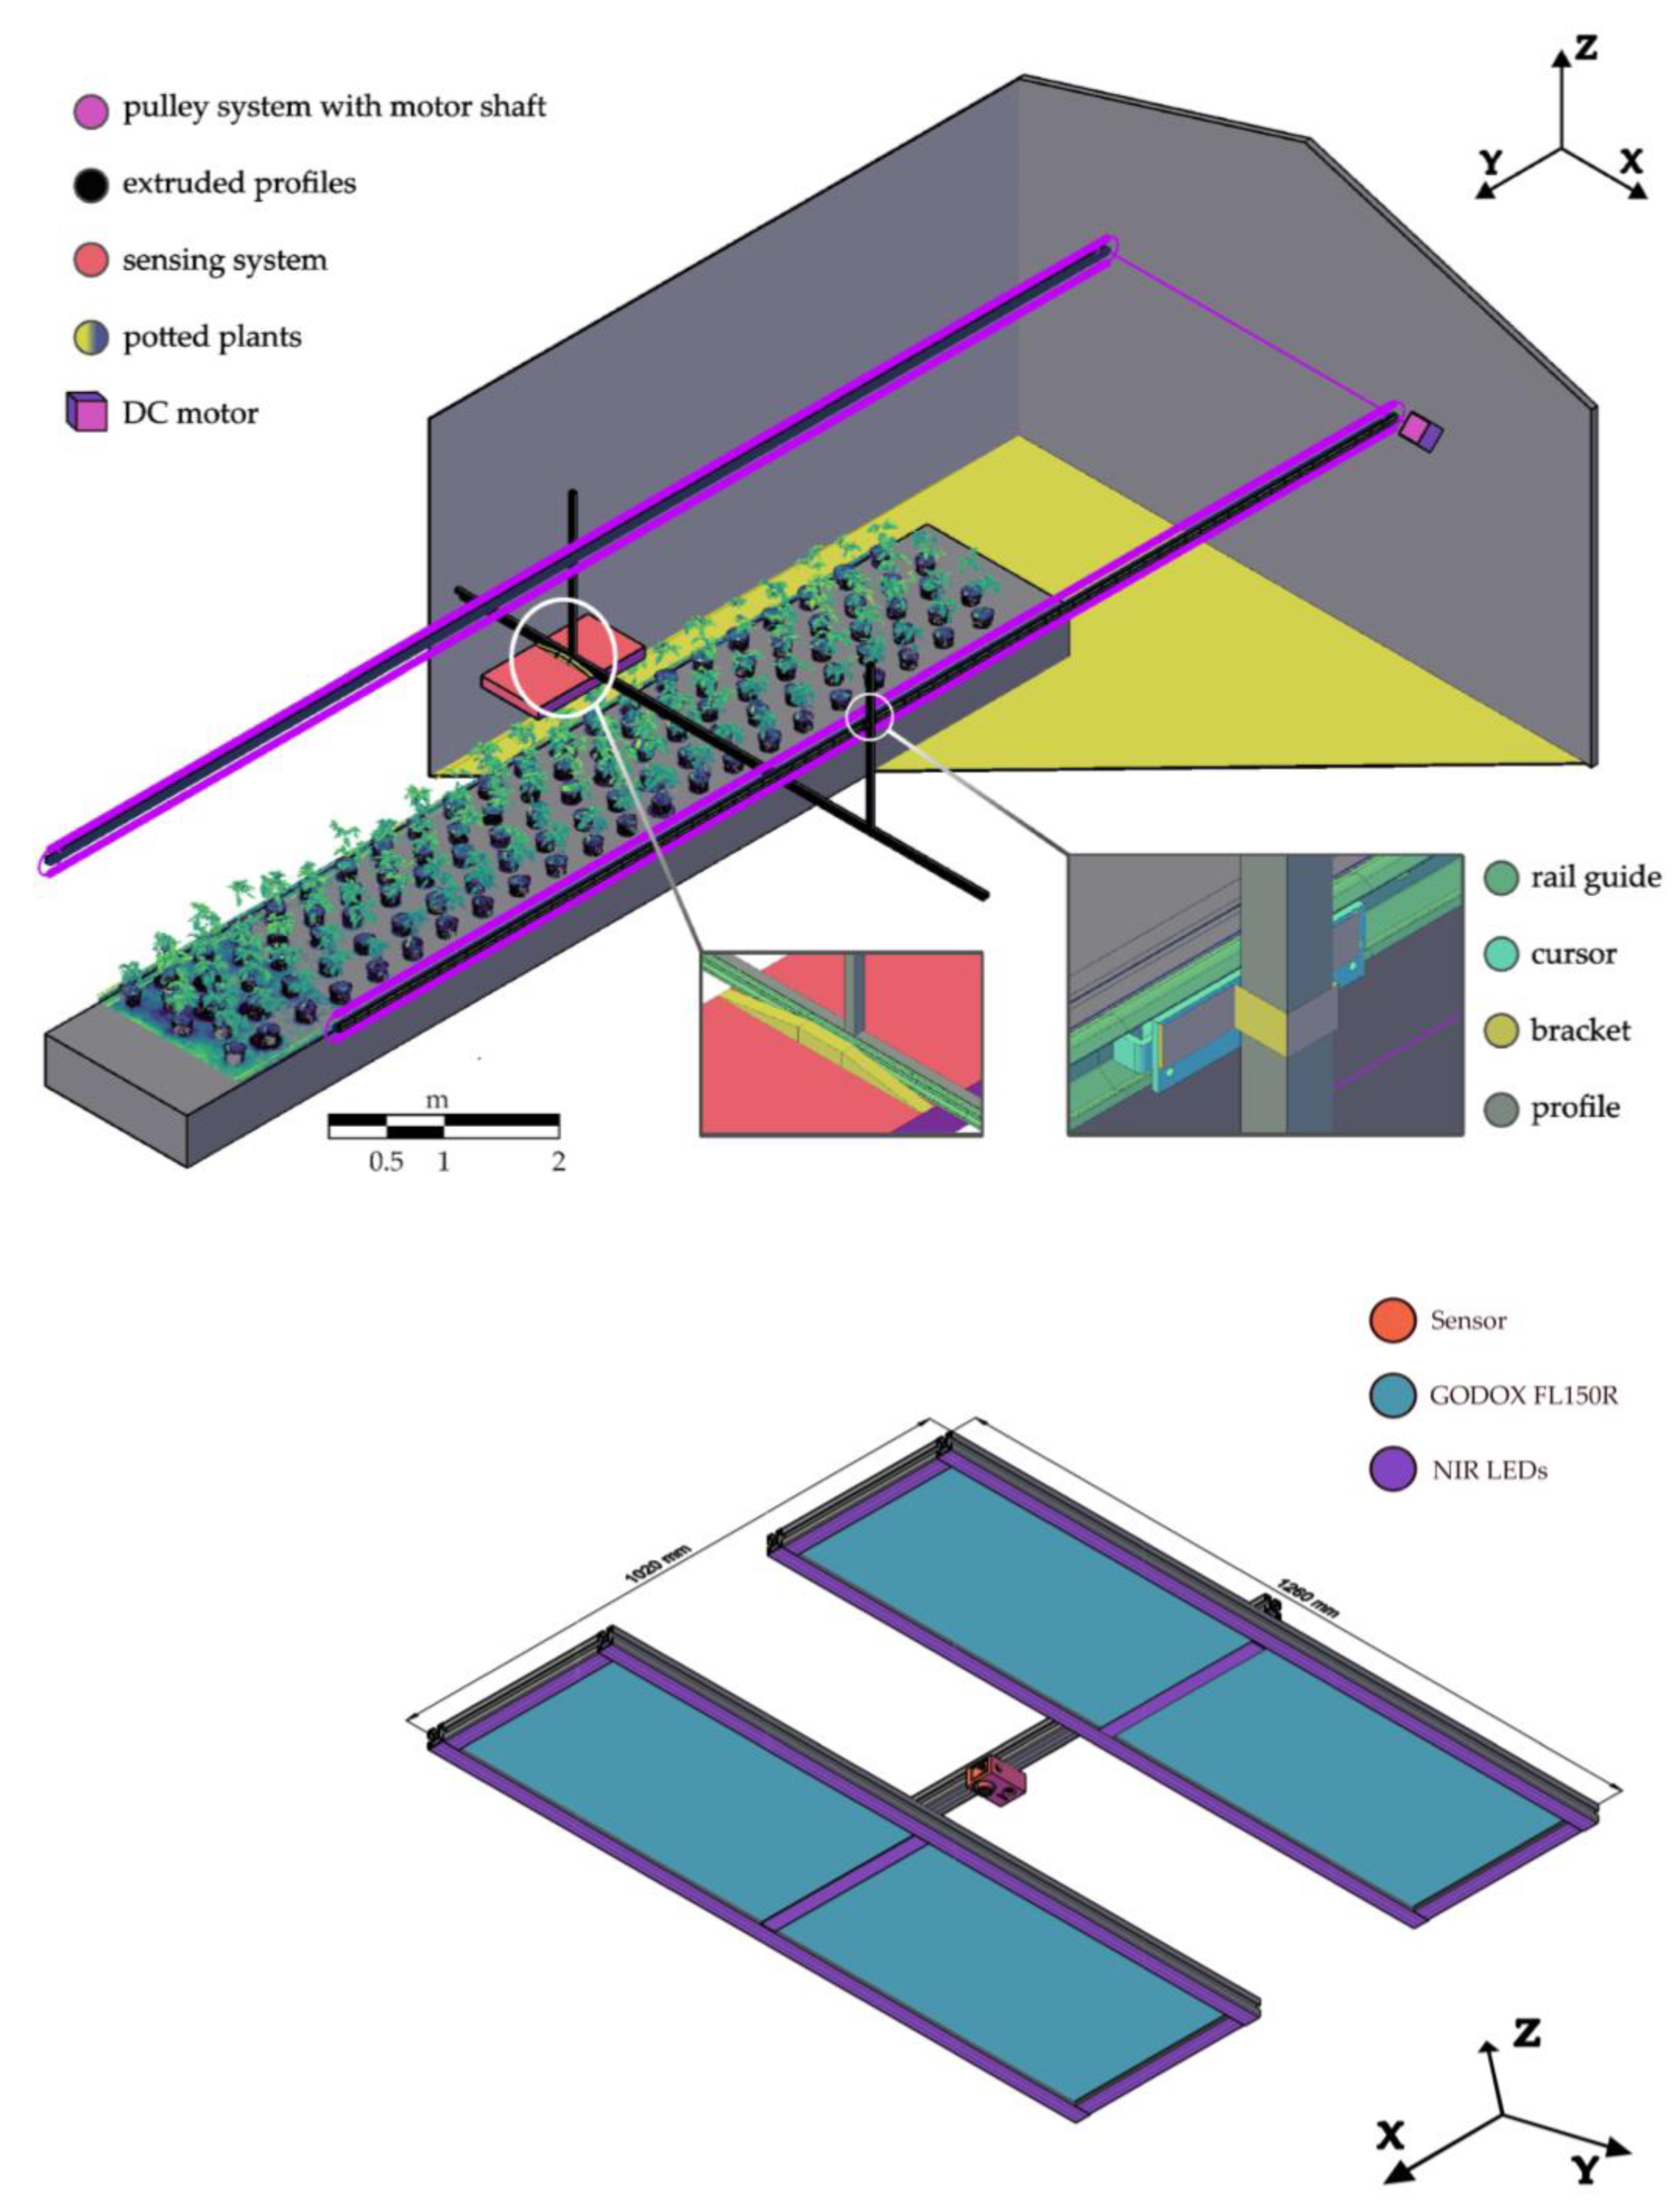
\includegraphics[width=\textwidth]{Images/agronomy-14-00306-g001}
    \caption{Platform and sensing system (top) and only the sensing system (bottom).}
    \label{fig:camera_position}
\end{figure}

Camera movement along the Y-axis in the greenhouse was controlled by a DC motor that operates through a pulley system. This system works similarly to a bridge crane that moves the imaging compound automatically with a speed of about 0.08 m/s along the Y-axis. The motion was manually activated and stopped.
The whole moving platform was made of (i) one MAPIR Survey3W (PeauProductions, San Diego, CA, USA) camera (S3) multispectral camera, (ii) two Light-Emitting Diode (LED) panels (GODOX FL150R) (Godox, Shenzhen, Guangdong, China) each measuring 1.2 × 0.3 m, and (iii) a 6-m LED strip emitting with a peak at 850 nm that encircles the GODOX FL150R panels to ensure that adequate Near-Infrared (NIR) radiation reaches the plants. Panels (the entire imaging system) ran parallelly to the bench hosting the pots to be imaged to ensure uniform illumination.
Furthermore, shading curtains were installed on the walls and ceiling of the greenhouse to reduce exterior light contribution during data collection.
A preliminary test was conducted to ensure the consistency of the spectrum provided by LEDs through its comparison with the reflectance spectrum acquired by an RS-5400 Spectroradiometer (Spectral Evolution, Haverhill, MA, USA). The acquisition was performed using calibrated panels of the RS-5400 instrument \cref{fig:spectral_signature} in lighting conditions replicating the operational environment.

\begin{figure}[H]
    \centering
    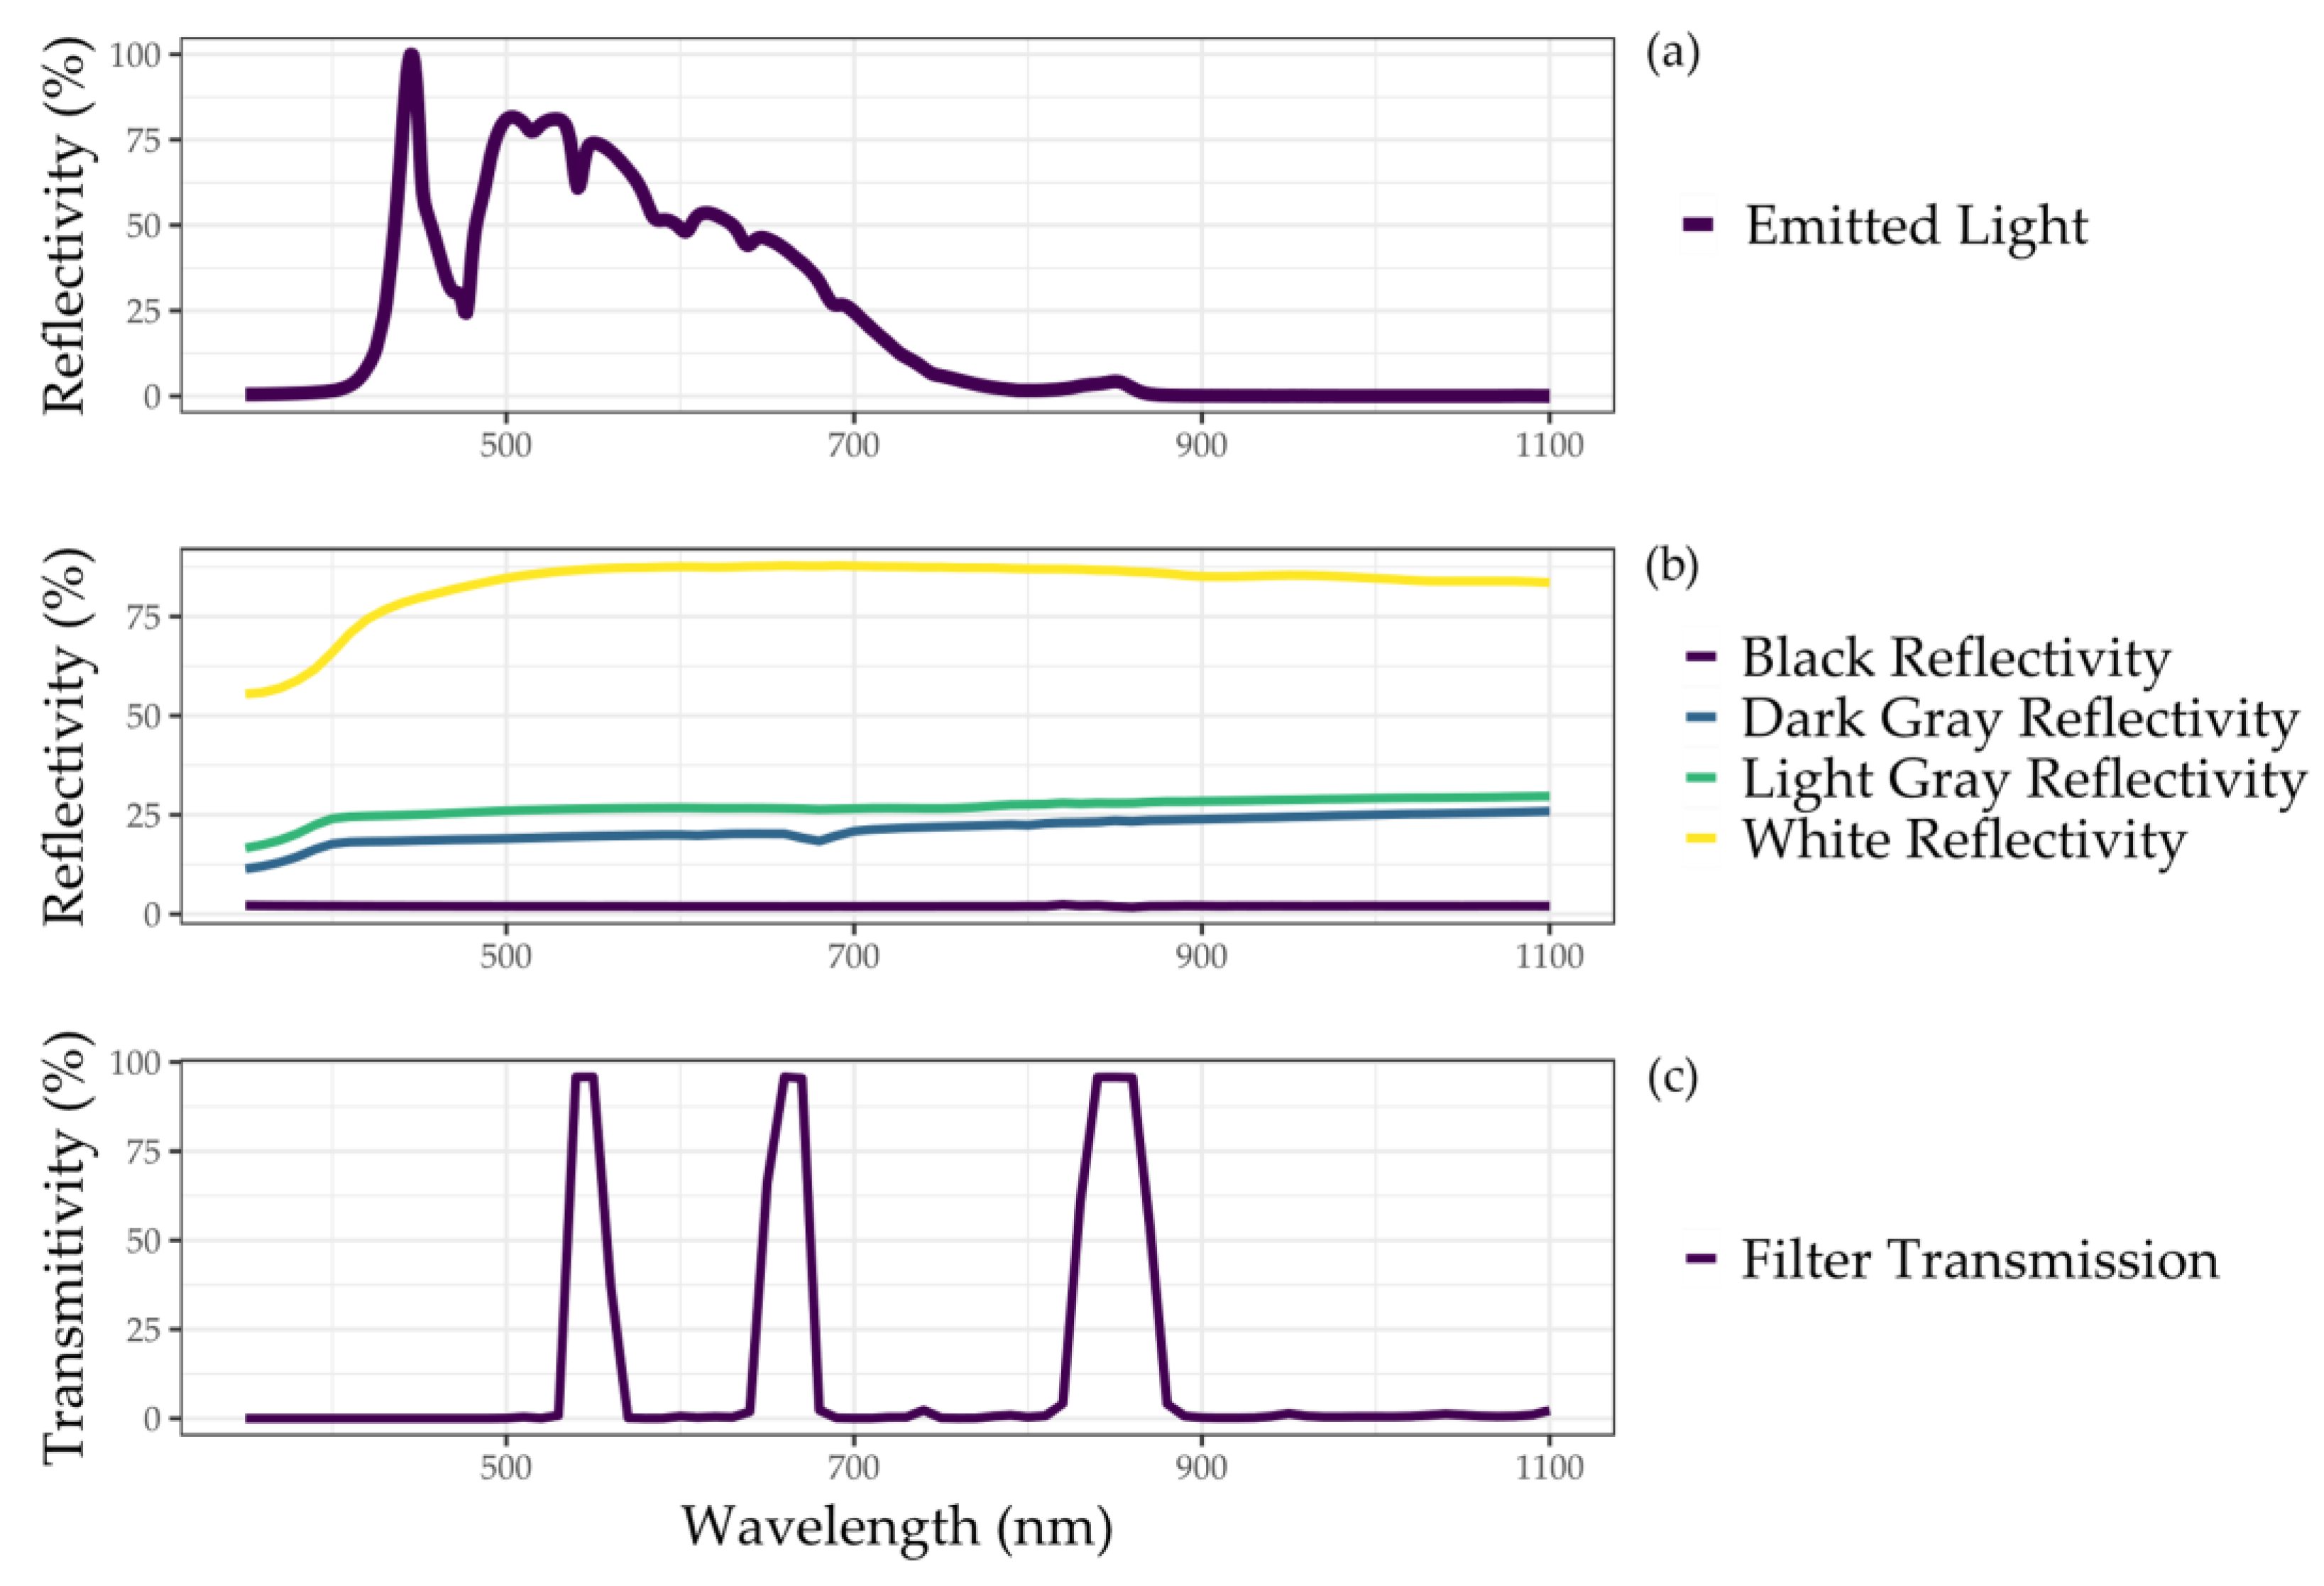
\includegraphics[width=\textwidth]{Images/agronomy-14-00306-g002}
    \caption{(a) Spectral signature of the reference panel, lighted with the tested LEDs and measured using the RS-5400 Spectro-radiometer. (b) Reflectivity of the MAPIR calibration panels corresponding to the different grayscale levels (yellow, light-green, blue, and violet colors in the graph) provided by the factory. The dark green line shows the filter sensitivity of MAPIR for the different bands. (c) Transmissivity of the S3 camera filter.}
    \label{fig:spectral_signature}
\end{figure}

The S3 camera was used for image capture, as detailed in \cref{tab:system_specifics}. A white balance setting was employed during acquisition to increase the intensity of the Red and NIR bands, resulting in a reduction of green band sensitivity.

\begin{table}[H]
\centering
\caption{S3 and system integration specifics.}
\begin{tabular}{p{5cm} p{5cm}}
\toprule
\textbf{Parameter} & \textbf{Value} \\
\midrule
Focal Length & 3.37 mm \\
Aperture & f/2.8 (fixed) \\
Lens Distortion & <1\% \\
Focal Length & Fixed \\
Hyper-focal Distance & 81.5 cm \\
Sensor Size & 3000 × 4000 pixels \\
Pixel Physical Size	& 1.55 μm \\
Bands & Green, Red, and NIR (Figure 2c) \\
Camera Shift (Y-axis)	& 20.3 cm per shot \\
Frames per second	& ~1/3 \\
Horizontal Footprint\textsuperscript{1}	& 202–276 cm \\
Vertical Footprint\textsuperscript{1}	& 152–207 cm \\
\bottomrule
\label{tab:system_specifics}
\end{tabular}
\footnotesize{\textsuperscript{1} at a 1.1–1.5 m distance.}
\end{table}

\subsection{Experimental Design}

An experiment was conducted to assess the reliability of the system and the processing workflow with respect to EPPO standards. The selectivity of a herbicide with an unknown mode of action was tested in a controlled environment greenhouse following EPPO standards 
\cite{PP11352014,DesignAnalysisEfficacy2012,PP13192021,PP11812022}. This allowed uniform growing conditions to be maintained throughout the greenhouse. Forty-four pots, each 40 × 30 cm, were sown with oilseed rape (OSR) and treated with the experimental product before emergence. The treatments were applied using an automatic spray chamber. To ensure a balanced set of PHYGEN, different concentrations of the herbicide, including a control group, were used to cover a range of phytotoxicity intensities. Visual and digital evaluations were carried out simultaneously. The PHYGEN assessment values were recorded as Day After Treatment (DAA) in
\cref{tab:PHYGEN_observations}.

\begin{table}[H]
    \centering
    \caption{PHYGEN observations.}
    \begin{threeparttable}
    \begin{tabular}{p{3cm}ccccc}
    \toprule
    \textbf{DAA\textsuperscript{1}} & \textbf{0\%} & \textbf{13\%} & \textbf{38\%} & \textbf{63\%} & \textbf{88\%} \\
    \midrule
    3 & 11 & 9 & 8 & 7 & 9 \\
    7 & 5 & 4 & 15 & 10 & 10 \\
    14 & 15 & 14 & 9 & 6 & 0 \\
    TOT & 31 & 27 & 32 & 23 & 19 \\
    \bottomrule
    \end{tabular}
    \begin{tablenotes}
    \item[1] Days After Application.
    \end{tablenotes}
    \end{threeparttable}
    \label{tab:PHYGEN_observations}
\end{table}

Only five discrete PHYGEN values were retained for scoring: 0\%, 13\%, 38\%, 63\%, and 88\%. This emphasizes the nature of the data generated by the visual assessment and the extreme use of the discrete quantitative scale. It is important to note that all five values were assigned during the three assessments, except on the last day, when the highest value (88\%) was not observed. This resulted in an imperfectly balanced distribution of PHYGEN over time. The interval between consecutive discrete values was 25\%, except for the interval between 0\% and 13\%. The 0\% value may be unreliable for treated pots due to the inevitable effect of herbicides, even for resistant crops. The true value in the range between 0\% and 13\% is difficult to detect, even for expert experimenters upon visual inspection, and is usually interpreted as having no effect on the harvest. Despite this, 0\% values were always recorded, as assessed by the experimenters.

\subsection{Data Processing}

The workflow starts with planning the image acquisition of the experimental plants. Then, the images are used to retrieve the multispectral 3D reconstruction of the plants. The parameters of the observed plants are extracted by the 3D model. Finally, the ML model is trained on the extracted parameters and validated. The workflow is summarized in
\cref{fig:workflow}.

\begin{figure}[H]
    \centering
    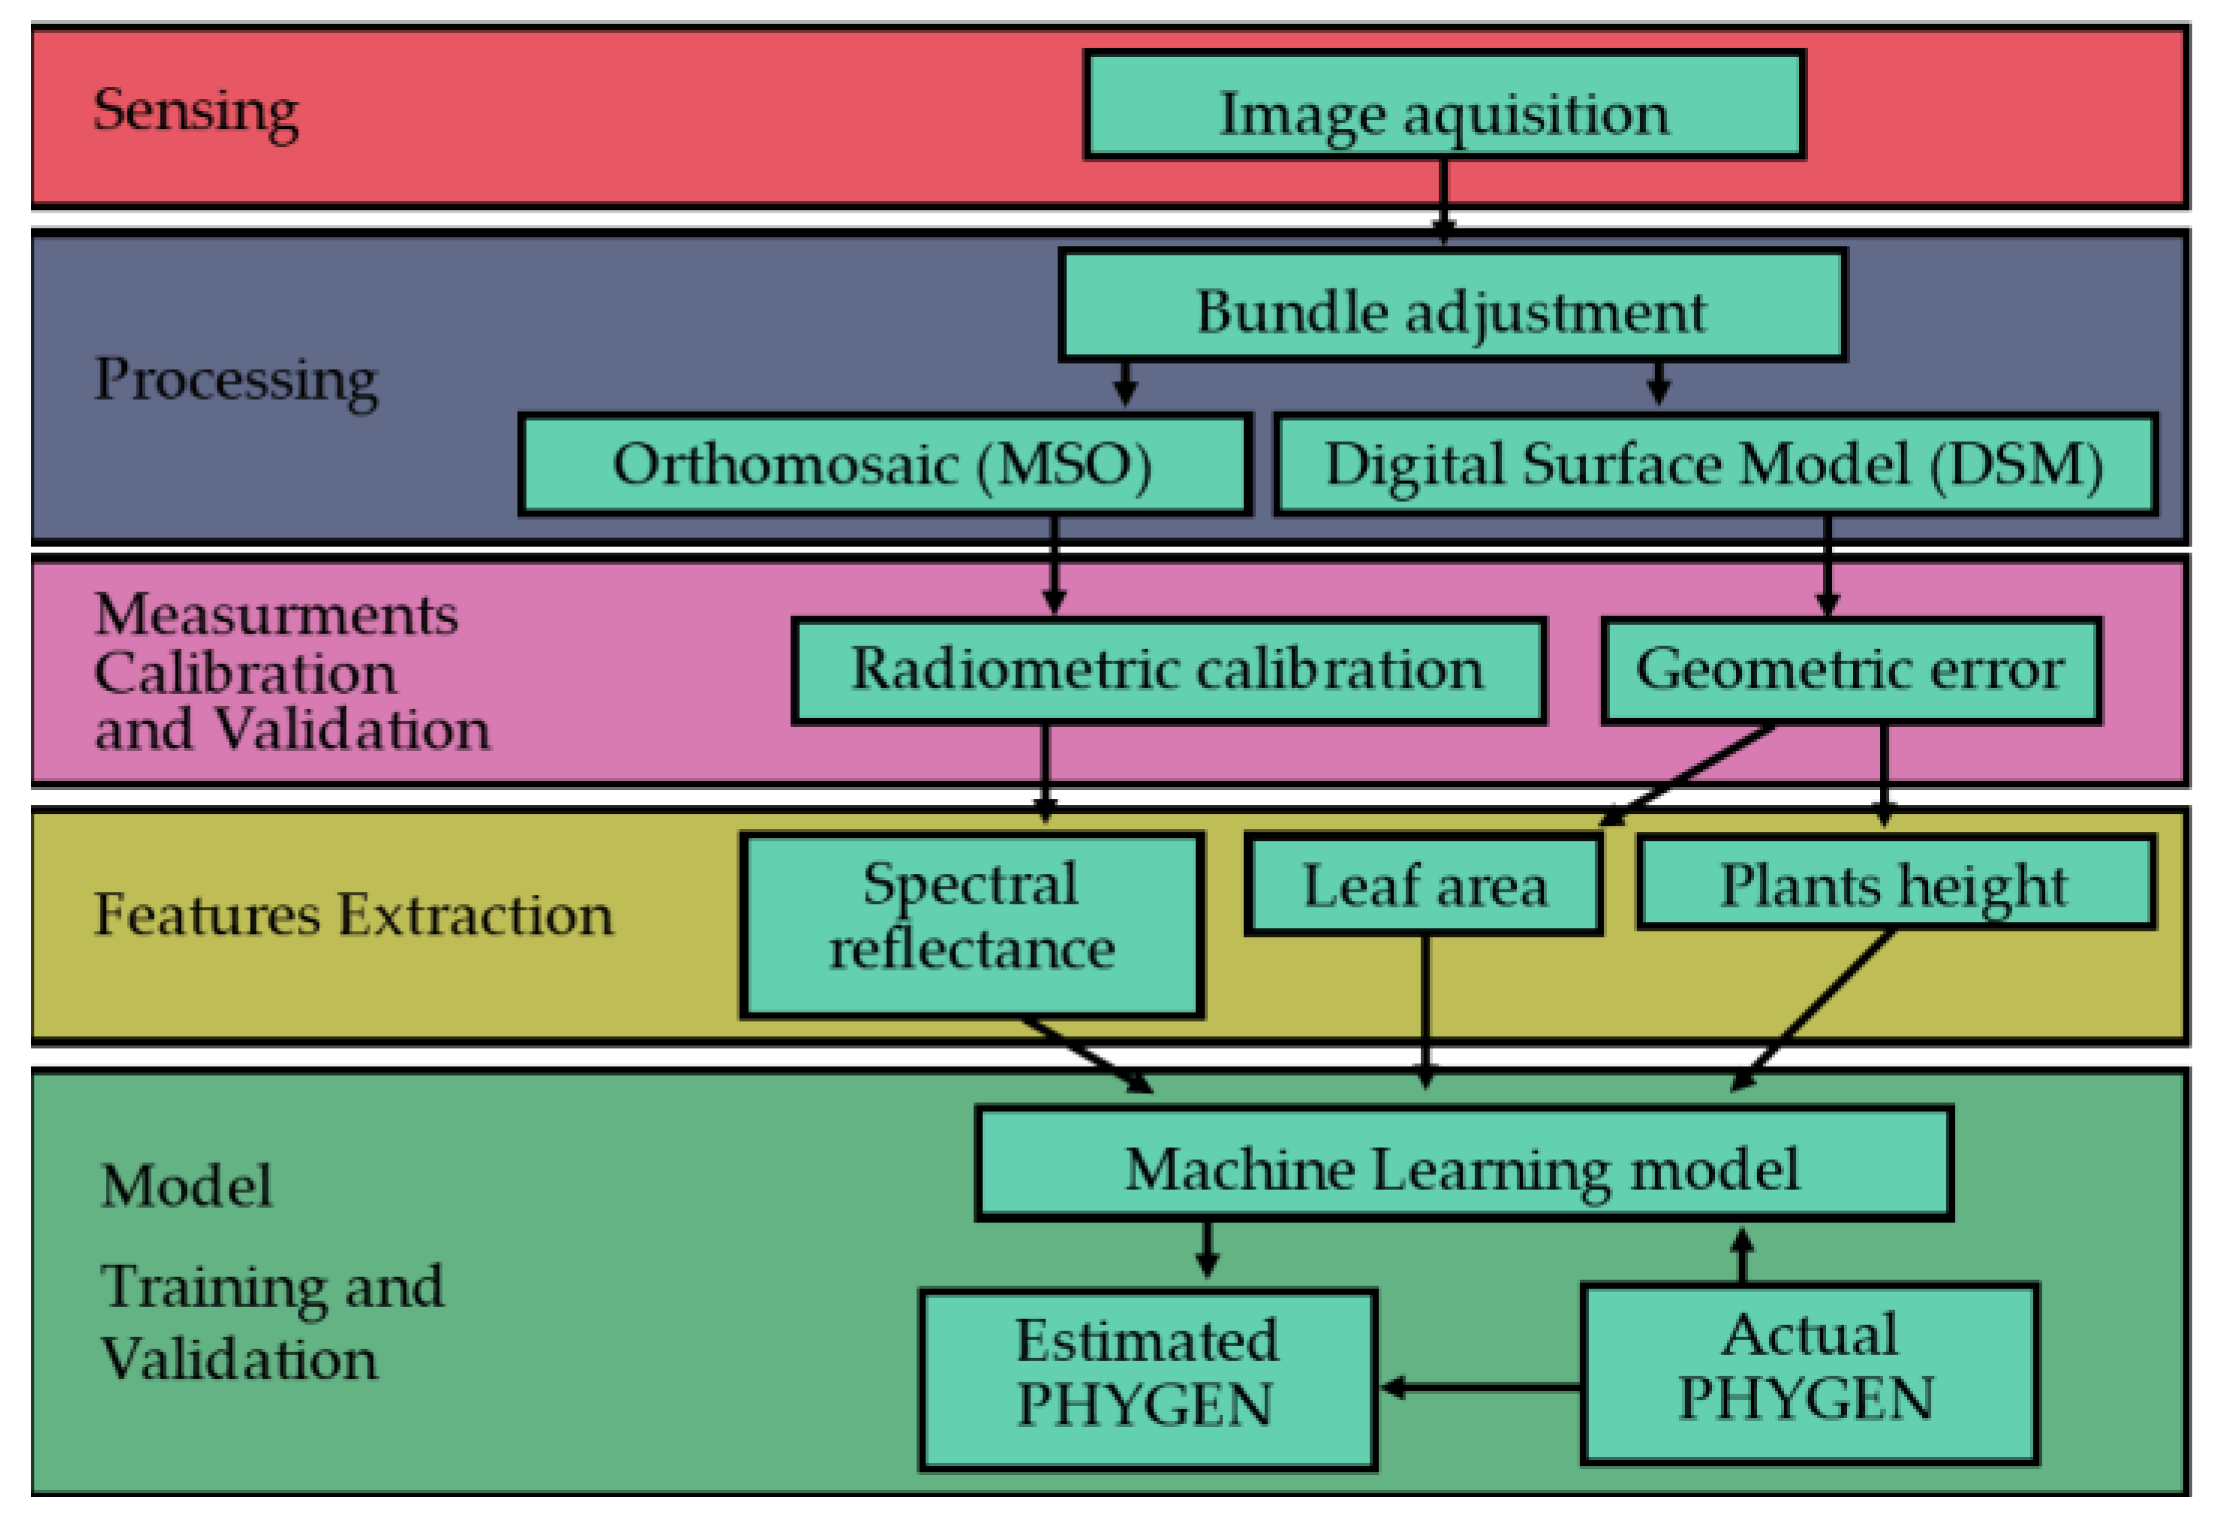
\includegraphics[width=\textwidth]{Images/agronomy-14-00306-g003}
    \caption{General workflow of the suggested method.}
    \label{fig:workflow}
\end{figure}

\subsection{Planning the Acquisition}

The camera movements were planned to capture stereoscopic images using a local Euclidean coordinate system, hereinafter called Coordinate Reference System (CRS), having the origin located at the lower left corner of the bench hosting plants.
Image block bundle adjustment was intended to refine both position and attitude image Exterior Orientation (EO) parameters, using nominal coordinates of the focal point position and a nadiral orientation as an initial solution during the adjustment.
Nominal values for image focal point position (X0, Y0, Z0) were determined assuming (i) X0 as the horizontal distance between adjacent strips; (ii) Y0 was computed by considering the speed of the camera shifts along the bars, and (iii) Z0 was set to a fixed value, which is discussed in the next paragraph. The camera was positioned with the longer side (4000 pixels) aligned across the track.
The nominal Z0 value was determined based on two conditions. First, the resulting image footprint must be consistent with the expected target size of plants. Second, targets should be visible at the smallest distance longer than the hyper-focal distance (0.815 m for S3). This condition ensures the maximum obtainable resolution, known as Ground Sampling Distance (GSD), which maximizes the efficiency and quality of tie point recognition. It is important to note that GSD is proportional to the physical pixel size according to
\cref{eq:GSD}.

\begin{equation}
    GSD = \delta \frac{H}{f}
    \label{eq:GSD}
\end{equation}

where H is the camera-to-target distance, f is the camera focal length, and $\delta$
 is the physical pixel size. As the height of the assessed plants can vary greatly during the same acquisition, H can range from 0.815 to 1.500, resulting in a ground sample distance (GSD) that varies between 0.37 and 0.69 mm·pixel\textsuperscript{-1}.

When planning an acquisition, it is important to ensure that the coarser GSD (which depends on H) is smaller than the smallest feature that needs to be recognized.
Tie point recognition depends on both the forward and side overlap among images. The forward overlap is determined by the baseline (B), which is the distance between consecutive focal points along the same strip. On the other hand, the side overlap is determined by the distance between two adjacent strips.
The platform is designed to operate with a strip distance equal to the baseline (0.2 m), resulting in 95% forward overlap.
In digital photogrammetry, it is widely acknowledged that the Z coordinate of target points is the most critical to estimate accurately. Its precision can be evaluated using
\cref{eq:sigma_z} \cite{depetrisRPASbasedPhotogrammetrySupport2020,borgognomondinoMultitemporalImageCoregistration2015,krausPhotogrammetryGeometryImages2011}.

\begin{equation}
    \sigma_z = \frac{H^2}{Bf} \sigma_x
    \label{eq:sigma_z}
\end{equation}

where H is the camera-target distance, $\sigma_x$ is the precision of parallax measures in the image domain (assumed to be half the physical pixel size, i.e., 1.685 μm for S3), B is the baseline, f is the sensor focal length, and 
$\sigma_z$ is the estimated precision of the Z coordinate of the target point.
The graphs in \cref{fig:base_effect} relate the theoretical (expected) $\sigma_z$ with the baseline $B$
while varying the camera-to-target distance at three reference values. The $B$
interval was considered to be within the minimum and maximum overlap.

\begin{figure}[H]
    \centering
    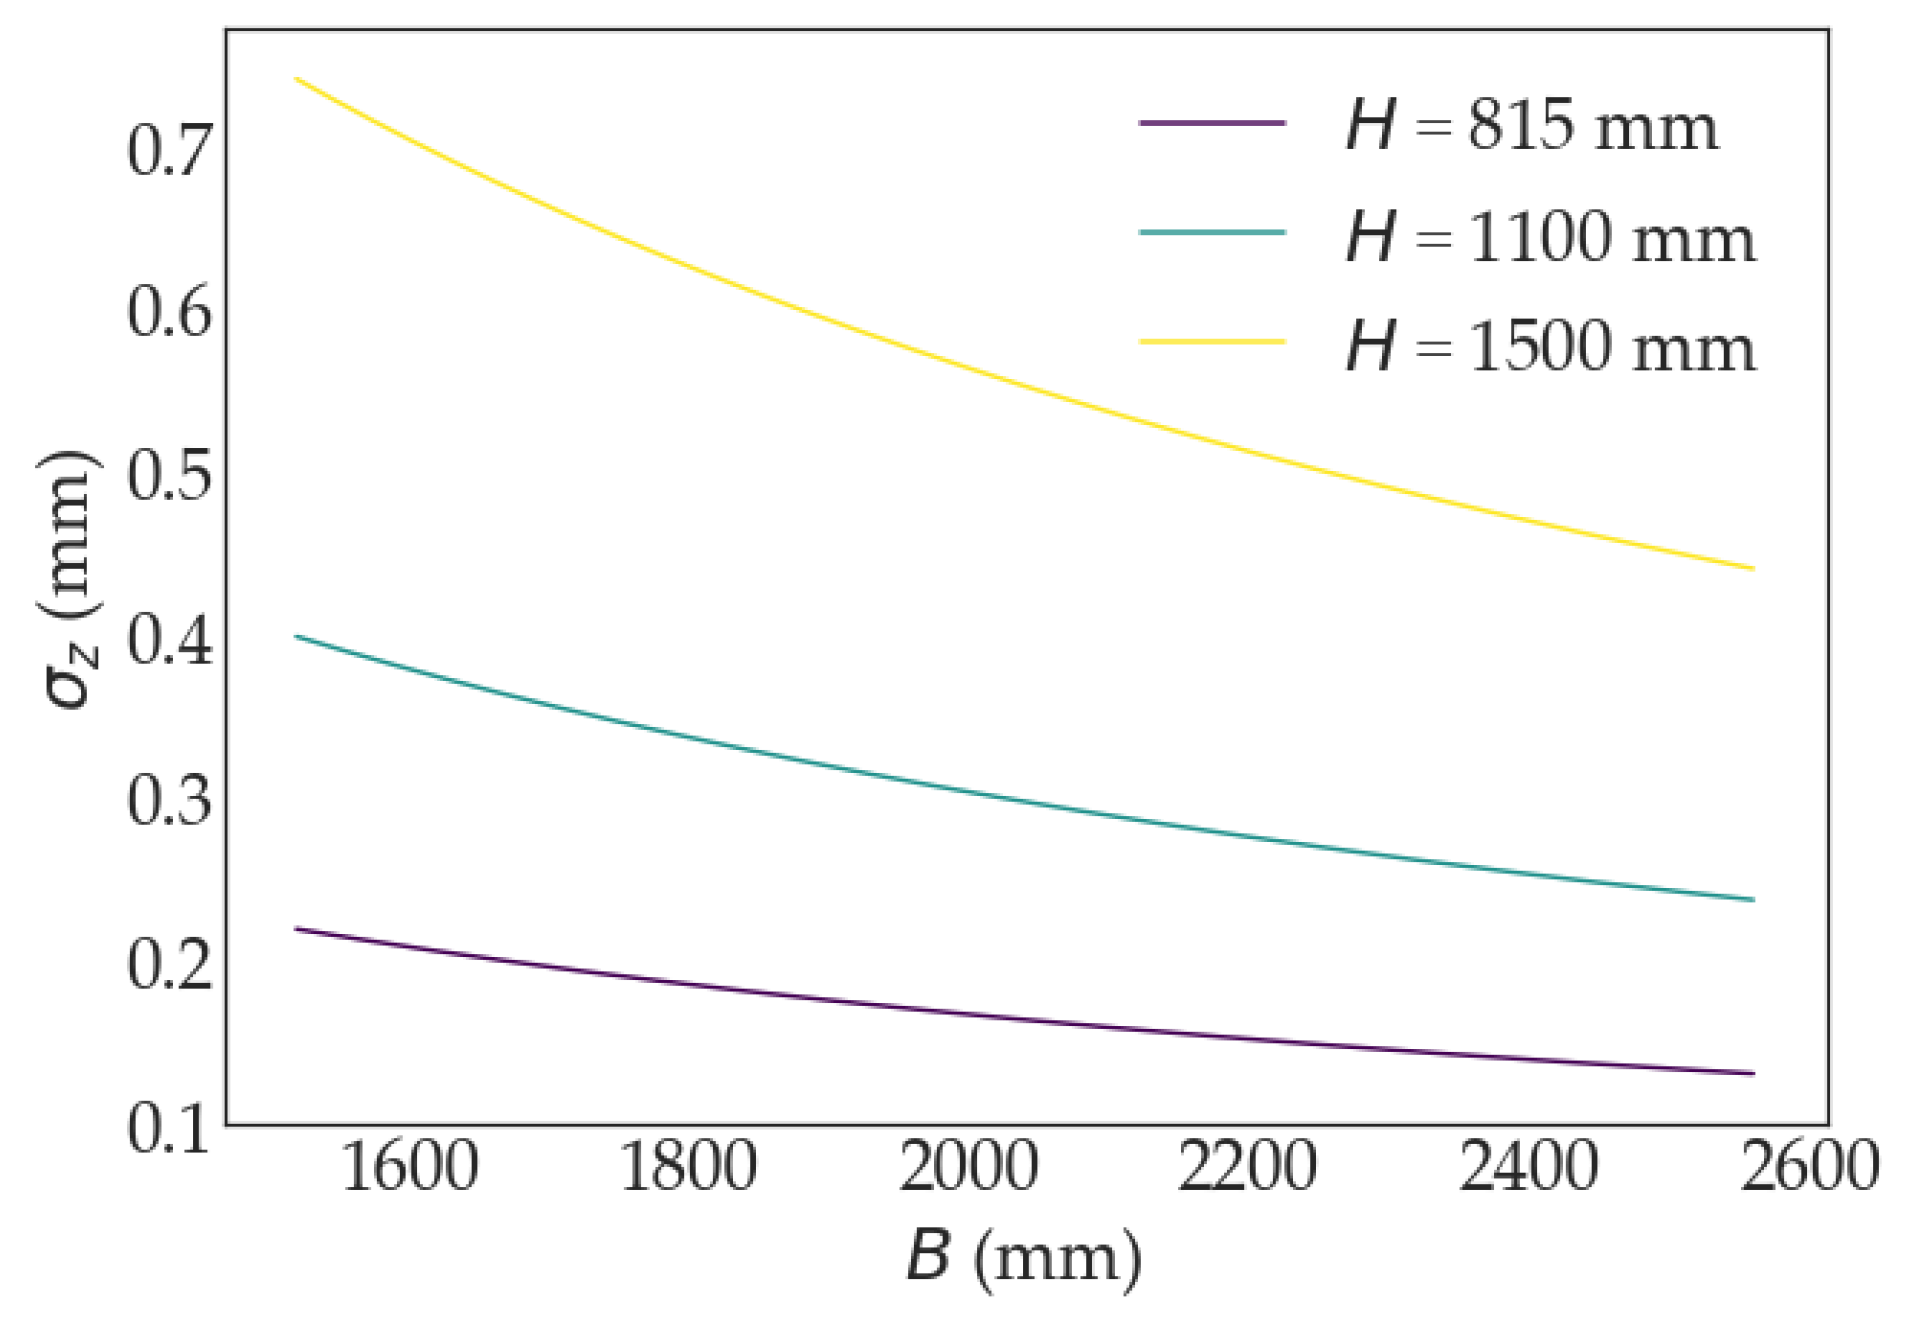
\includegraphics[width=\textwidth]{Images/agronomy-14-00306-g004}
    \caption{$\sigma_z$ estimates computed by \cref{eq:sigma_z}. Colored curves refer to different D values.}
    \label{fig:base_effect}
\end{figure}

\cref{eq:sigma_z} was used to estimate the actual Z precision from the bundle adjustment solution and compare it to the expected (theoretical) precision
($\sigma_z$).
To enhance the robustness of validation and test for geometrical errors, four metered tapes were placed over the bench
(\cref{fig:Geometric_calibration}), and at least nine GCPs were manually positioned throughout the scene for each acquisition date. The GCPs were positioned in a pattern to ensure a uniform distribution across the image block in both longitude and latitude. The GCPs were at three different heights: 0 m, 0.35 m, and 0.7 m.

\begin{figure}[H]
    \centering
    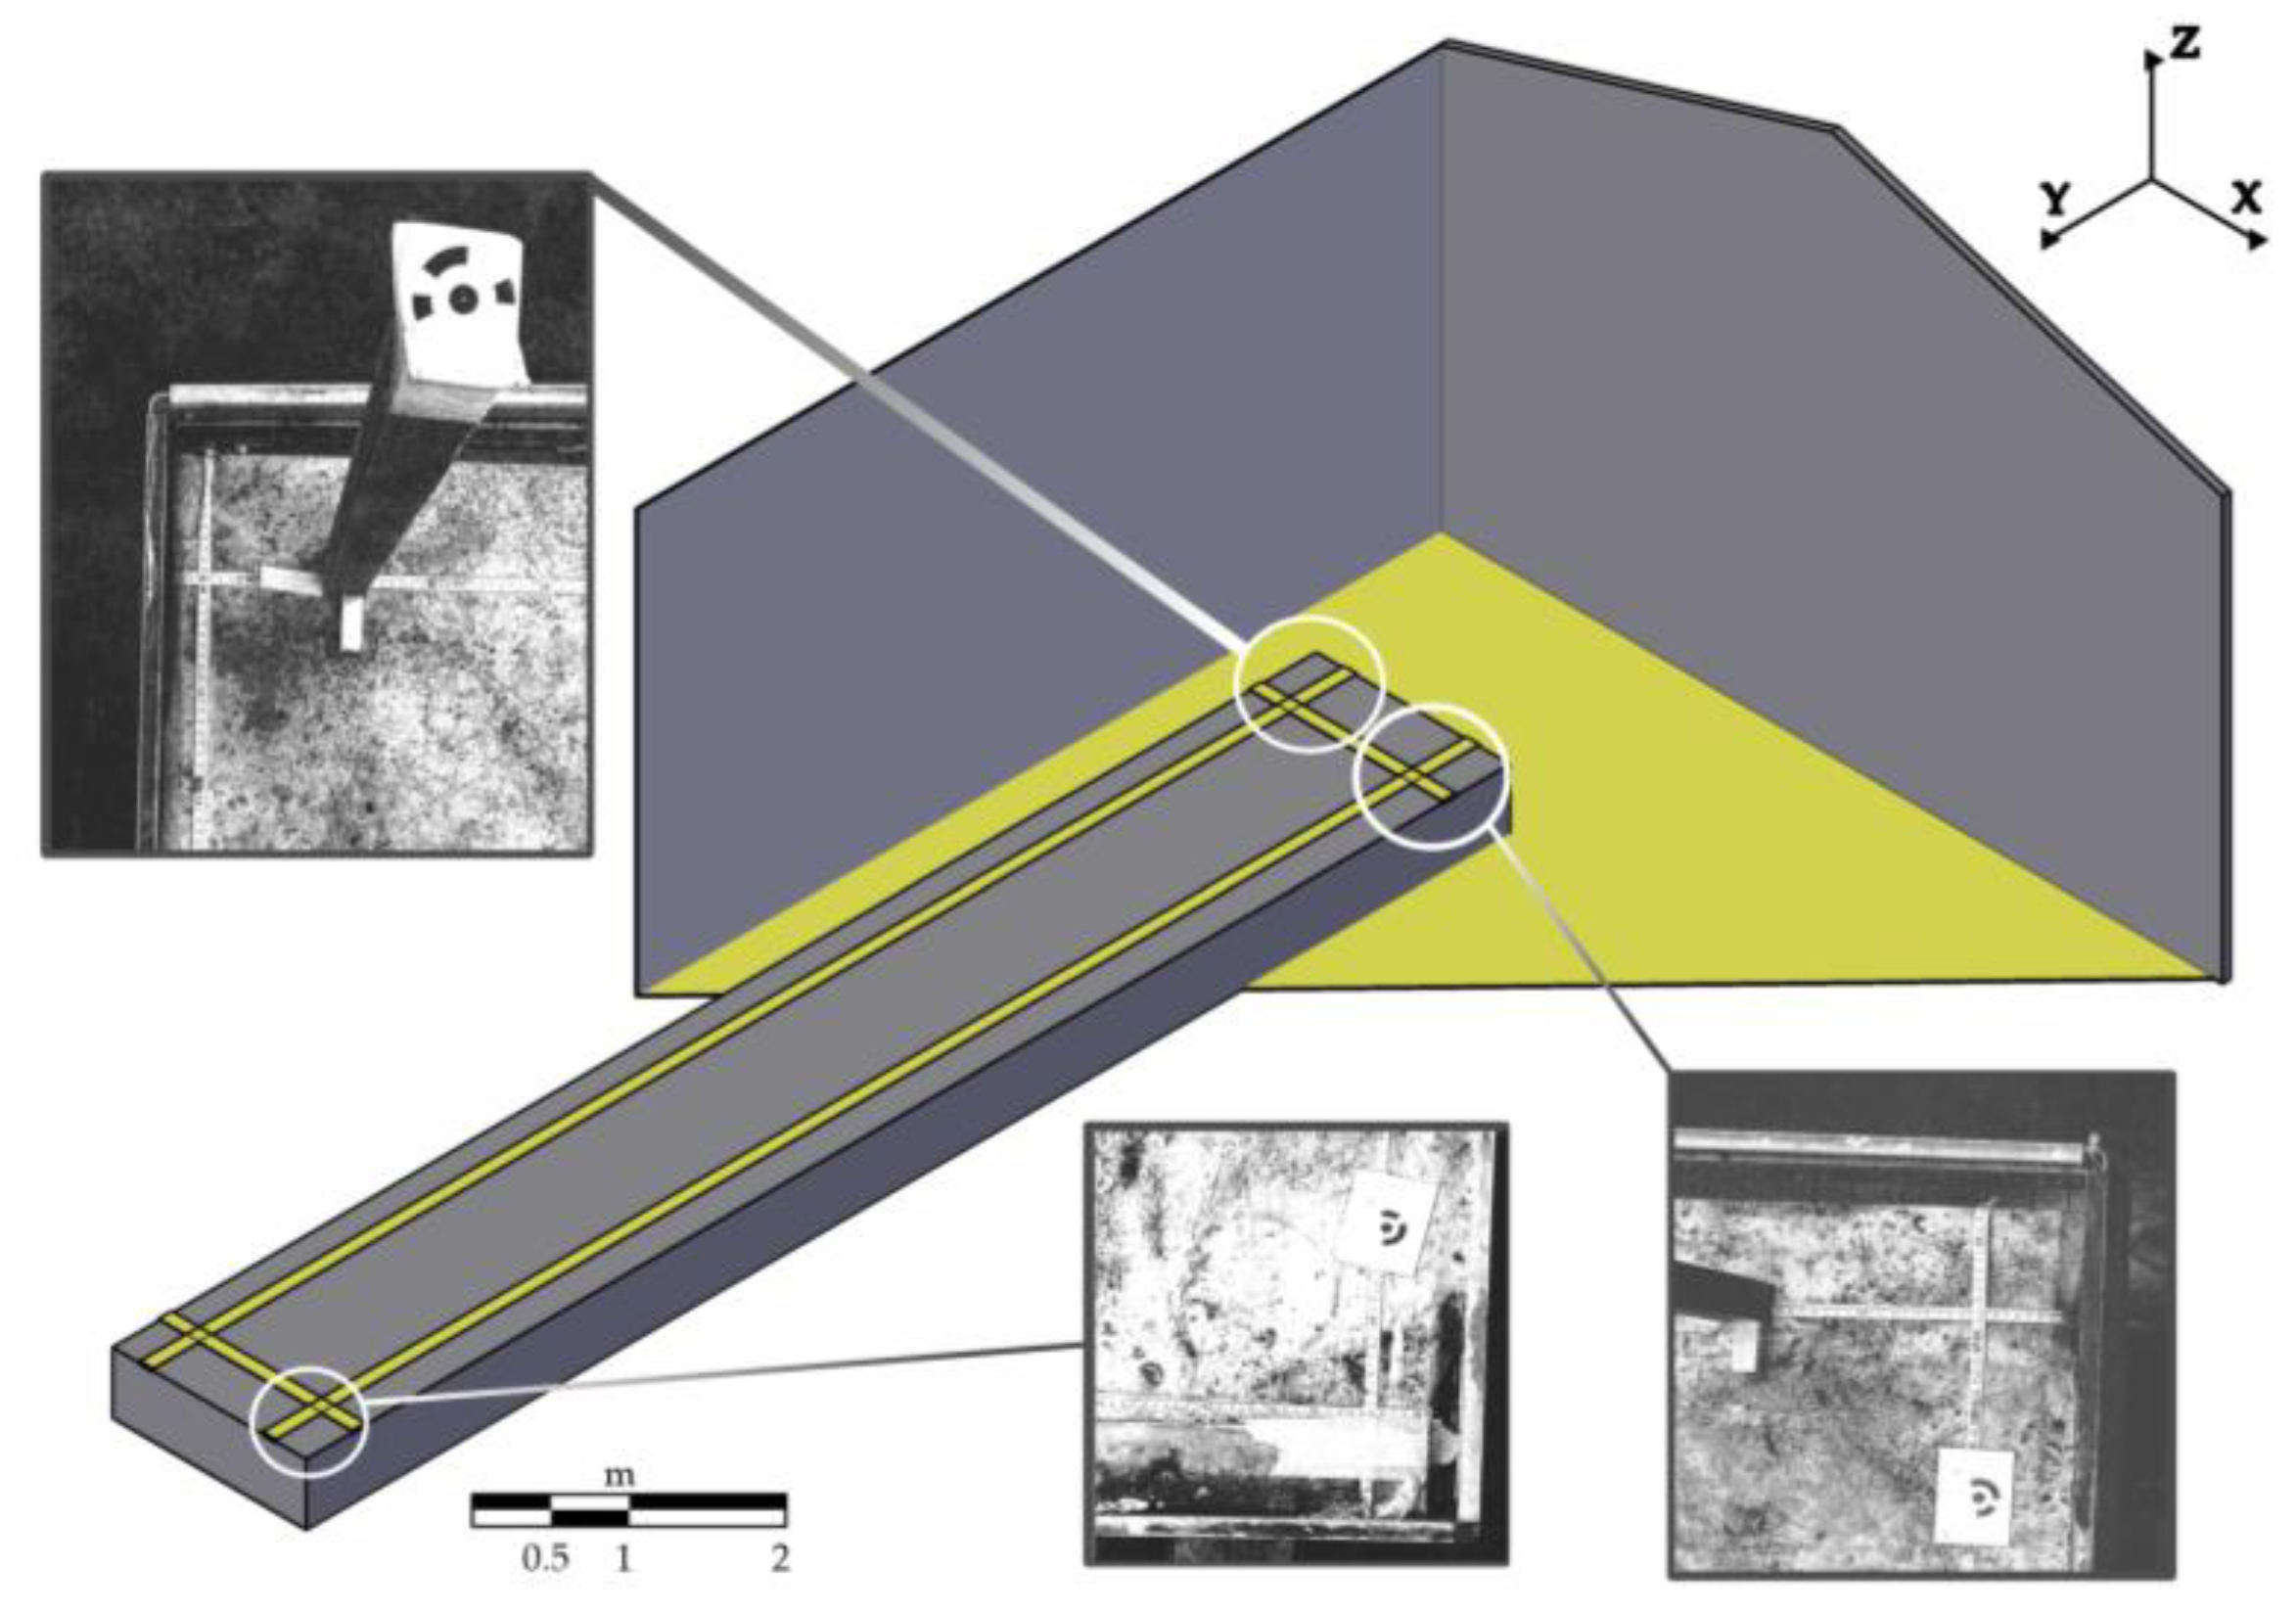
\includegraphics[width=\textwidth]{Images/agronomy-14-00306-g005}
    \caption{Metered tapes and GCPs on the bench.}
    \label{fig:Geometric_calibration}
\end{figure}

In summary, the only adjustable parameters for planning the acquisition were (i) the Z position of the camera and (ii) the distance between strips (side overlap). The Z position was set at 1.5 m from the bench, and the distance between strips (on the X axis) was 20 cm in all three assessments.

\subsection{Bundle Adjustment and Point Cloud Generation}

Digital photogrammetry software utilize computer vision algorithms, such as the Scale-Invariant Feature Transform (SIFT), to automatically identify potential tie points in images
\cite{oteroAnatomySIFTMethod2014,loweDistinctiveImageFeatures2004,loweObjectRecognitionLocal1999}.
Photogrammetric software may use various algorithms to match these points across images, including Random Sample Consensus (RANSAC) or other methods, depending on computational efficiency and accuracy requirements
\cite{FASTAPPROXIMATENEAREST2009}.
After matching the points, software uses bundle adjustment to estimate the spatial locations of the points and the camera positions. This process takes into account the matched points and the camera’s Exterior and Interior Orientation (EO/IO) parameters
\cite{krausPhotogrammetryGeometryImages2011,hartleyMultipleViewGeometry2004,gomarascaElementsPhotogrammetry2009}.
This study employed tie point identification, matching, and bundle adjustment using Agisoft Metashape version 2.1.0 (Agisoft LLC, St. Petersburg, Russia). To support image bundle adjustment, a portion of the GCPs and initial camera EO/IO parameters were provided
\cite{atkinsonCloseRangePhotogrammetry1996,triggsBundleAdjustmentModern2000,moulonPositionnementRobustePrecis}.
As far as IO parameters are concerned, the initial values used to bootstrap adjustment were the following: (i) focal length as supplied by S3 and (ii) lens distortion parameters = 0, coordinates of the Principal Point of Autocollimation (PPA) equal to the physical center of the image (fiducial point). Sensor array and physical pixel size were set to their nominal values.
The solution was spatially referenced using GCP coordinates, which are referred to as a local reference system (CRS). The resulting point cloud associates spectral values from bands to each point. These values were obtained as the mean value of the image pixels corresponding to the target points. Bundle adjustment provides estimated camera EO and IO parameters and their uncertainties, as well as all GCP coordinates estimated by the model and their corresponding errors. The GCPs involved in the bundle adjustment allow for the detection of outliers and refinement of the solution by running the bundle adjustment again after removing the outliers.
To ensure accuracy, the solution was checked by three GCPs, which were not involved in bundle adjustment. The adjustment solution was considered satisfactory if the difference between these three GCP values from the model and the reference values was less than or equal to the expected error.

\subsection{Products}

A digital surface model (DSM) with a GSD inherited from the previous steps was generated from the point cloud data. The DSM was then utilized to create the final multi-spectral orthomosaic (MSO)
\cite{gomarascaElementsPhotogrammetry2009}.
Both the DSM and MSO are projected in the CRS.

\subsection{Radiometric Calibration of the Multi-Spectral Orthomosaic}

MSO radiometric calibration was performed using an empirical line approach with reference reflectance values obtained from the S3 calibrated panel provided by the MAPIR company
\cite{MAPIR_Survey3_Camera_Datasheet_Englishpdf}.
The average pixel value from each squared area of the panel having the same grey level was computed for all the bands of the non-calibrated orthomosaic.
Reference reflectance values from the MAPIR calibration panel were compared with the averaged ones from the orthomosaic by scatterplot. An Ordinary Least Squares approach was used to calibrate a linear function modeling the relationship between MSO Digital Numbers and the correspondent “expected” reflectance values
\cite{cameraMAPIRCameraReflectance}.
Calibration function definition was carried out separately for each band.
The resulting functions were then applied to all the pixels of MSO bands, resulting in a calibrated (reflectance) version of MSO
\cref{fig:mask}.

\begin{figure}[H]
    \centering
    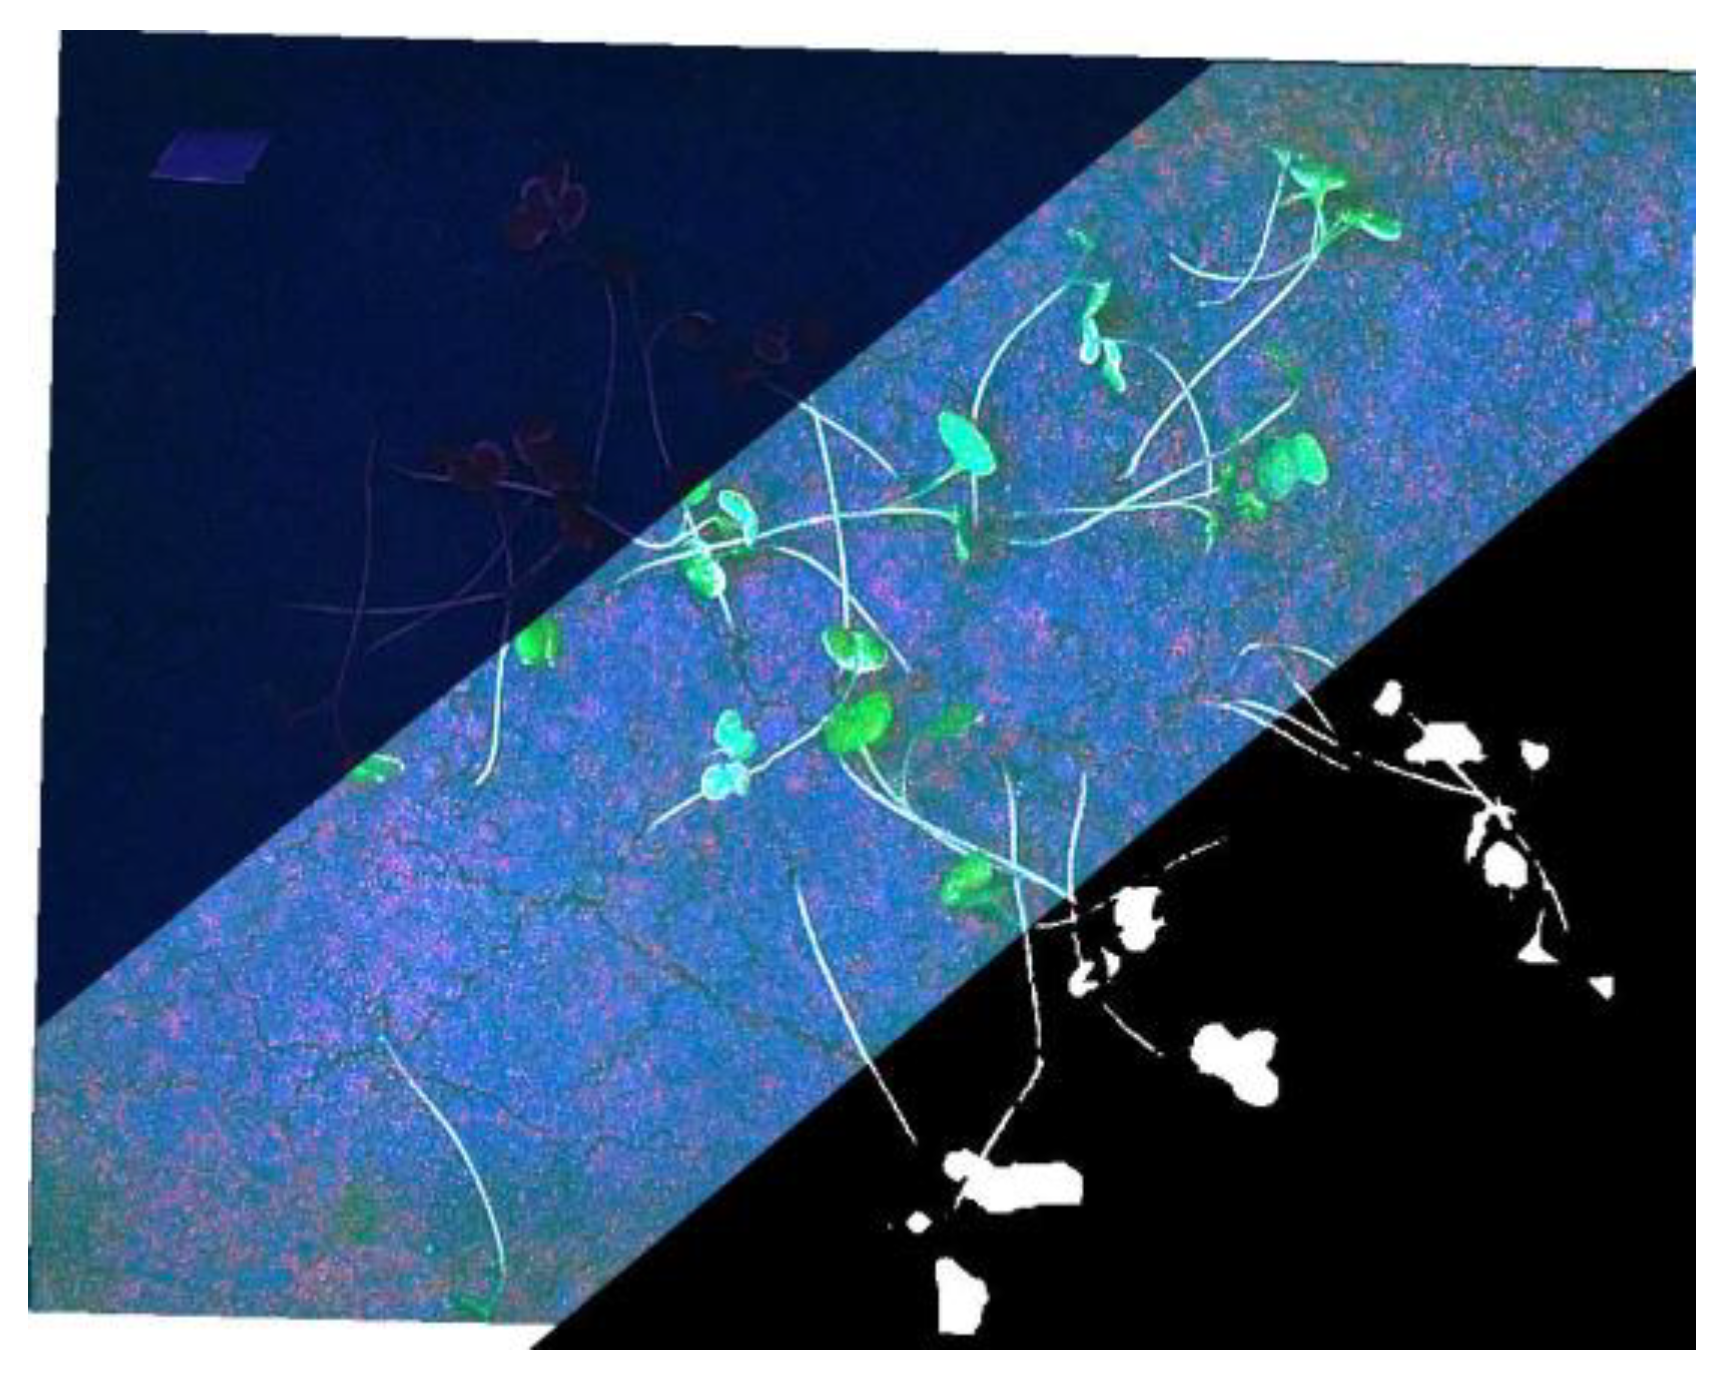
\includegraphics[width=\textwidth]{Images/agronomy-14-00306-g006}
    \caption{Non-calibrated (dark) and calibrated MSO are shown together with the last vegetation mask (white pixels) on an oil seed rape pot.}
    \label{fig:mask}
\end{figure}

The radiometric calibration accuracy was computed as the Mean Absolute Error (MAE) between the panel ground truth values and the forecasted values
\cite{wyattRadiometricCalibrationTheory2012} according to Equation

\begin{equation}
    MAE = \frac{\sum_{i=1}^{n} \left| y_i - x_i \right|}{n}
\end{equation}

where $y_i$  is the expected reflectance value of the i-calibration panel square,
$x_i$ the estimated correspondent one, and $n$ the number of observations.

\subsection{MSO Classification}

A vector format file was generated to map the area of each potted plant. A local coordinate system (CRS) was adopted. The file contains two essential pieces of information: a unique identifier for each plant and the date of assessment. The second process involved manually isolating the plant from the soil in the pot using thresholding, focusing only on the plant pixels. The soil was identified and masked by applying a bimodal threshold 
\cite{otsuThresholdSelectionMethod1979}.
to the green band. The mask was then refined using a semi-automatic technique
\cite{rotherGrabCutInteractiveForeground2004}.
This step produced the final vegetation mask (VM) \cref{fig:mask}, effectively isolating the plants for analysis.

\subsection{Predictors}

It is important to note that a PHYGEN estimate, in terms of a continuous variable, 
is the main expected outcome of this work. To achieve this task, the VM-derived 
area was assumed as a proxy for the Leaf Area Index (LAI). Differently, the mean (µ) 
and standard deviation ($\sigma$) of the following bands/indices from the calibrated S3 
orthomosaic were computed: (i) Red, Green, and NIR bands, (ii) Normalized Difference 
Vegetation Index (NDVI), and (iii) Soil Adjusted Vegetation Index (SAVI).
Additionally, the mean (µ) and standard deviation ($\sigma$) of heights of pixels 
belonging to VM were obtained by differencing DSM values of pixels within VM and 
the average of DSM values of soil pixels.
Finally, the date of acquisition (defined as DAA) was also considered to calibrate 
the prediction model.

\begin{table}[H]
    \centering
    \caption{Predictors and their meanings.}
    \begin{tabularx}{\textwidth}{XX}
    \toprule
    \textbf{Predictors} & \textbf{Variables meaning} \\
    \midrule
    (4) $NDVI = \frac{\rho_{NIR} - \rho_{RED}}{\rho_{NIR} + \rho_{RED}}$ & where $\rho_{NIR}$ and $\rho_{RED}$ are the calibrated reflectance values from MSO \\
    (5) $SAVI = \frac{1.5 \cdot (\rho_{NIR} - \rho_{RED})}{(\rho_{NIR} + \rho_{RED} + 0.5)}$ & where $\rho_{NIR}$ and $\rho_{RED}$ are the calibrated reflectance values from MSO \\
    (6) $H_P = H_V - \overline{H_S}$ & where $H_P$ is the computed pixel relative average height of the vegetation contained in a pot, $H_V$ is the absolute height of vegetation pixel in a pot, and $\overline{H_S}$ is the average absolute height of soil level in a pot. \\
    \bottomrule
    \end{tabularx}
    \label{tab:predictors}
\end{table}

\subsection{ML Model}

The available dataset is made of 132 multivariate observations (n), each providing 14 different predictors (p). To simplify the model and reduce parameters, the least absolute shrinkage and selection operator (LASSO) model (7) was used 
\cite{hastieElementsStatisticalLearning2009}.
The PHYGEN variable ($y$) originally expressed as a percentage, was transformed into a probability by dividing it by one hundred. As PHYGEN values range between 0 and 1, a linear regression model is unsuitable. A logistic function was used to adjust the linear predictions from the LASSO model to the PHYGEN scale, which is relevant to human vision.
Twelve variables from MSO and DAA were normalized and used as independent variables. The dataset was split into an 80\% training set and a 20\% testing set. A K-fold (K = 10) strategy was applied to train and cross-validate the model
\cite{jamesIntroductionStatisticalLearning2023}.
To ensure a balanced splitting of observations, a stratified method was used based on PHYGEN values and acquisition dates. The human visual PHYGEN was fitted using a multivariate regression model with a 
$L_1$ regularization term \cite{friedmanRegularizationPathsGeneralized2010} and a least squares adjusting method.
The hyperparameter $\lambda$ of $L_1$ was determined through a cross-validation involving 5 subsets of the training data, each representing a different part of a logarithmic range developing approximately between 0.003 and 0.67. The trained model outputs were then used as inputs for a logistic function (LF) (8), which was fitted to the PHYGEN data. The function parameters were estimated using non-linear least-squares optimizatio
\cite{garbowMINPACK1SubroutineLibrary1984,stornDifferentialEvolutionSimple1997},
with initial values inferred from the PHYGEN distribution. The optimization aimed to minimize two error functions in the model, thereby enhancing the accuracy of the PHYGEN prediction:

\begin{table}[H]
    \centering
    \caption{Models, their loss functions, and model outputs.}
    \begin{tabularx}{\textwidth}{XXX}
    \toprule
    \textbf{Model} & \textbf{Loss function} & \textbf{Model output} \\
    \midrule
    \textit{LASSO} & $\sum_{i=1}^{n} \left( y_i - \beta_0 - \sum_{j=1}^{p} \beta_j x_{ij} \right)^2 + L_1 = \min; L_1 = \lambda \sum_{j=1}^{p} |\beta_j|$ & $\hat{\beta}_j, \hat{\beta}_0$ (7) \\
    \textit{LogisticFunction (LF)} & $\sum_{i=1}^{n} \left( y_i - \frac{L}{1 + e^{-k(\hat{y}_i - y_0)}} \right) = \min$ & $\hat{L}, \hat{k}, \hat{y}_0$ (8) \\
    \bottomrule
    \end{tabularx}
    \label{tab:models}
\end{table}

where $y_i$  is the i-PHYGEN observed rate, $x_ij$ (7) is the observed value of the j-th explaining variable, 
$\beta_0$ (7) is the intercept of the function, $\beta_j$ (7) is the weight corresponding to j-th variable, and
$\hat{y_i}$  (8) is the predicted value of the PHYGEN rate computed using weights estimated values from LASSO
($\hat{\beta}_j$,$\hat{\beta}_0$).
The logistic function (8) has three parameters: $L$, $y_0$, and $k$.
These correspond to the higher limit of the function, the inflection point of the sigmoid, and the rate of growth, respectively. The estimated values for 
$L$, $k$, and $y_0$ are, respectively, $\hat{L}$, $\hat{k}$, and $\hat{y}_0$,
the correspondent estimated values. Initial values of $\hat{L}$, $\hat{k}$, and $\hat{y}_0$
, needed to run the not-linear least squares were set to 100, 50, and a random value extracted in the range [0, 1], respectively.

\section{Results and Discussion}

\subsection{Measurement Errors}

The surveyed 3D coordinates of GCPs were compared to those obtained from the photogrammetric restitution of the adjusted image block to assess errors associated with geometric features. To ensure a reasonable level of robustness for the accuracy assessment despite the low number of surveyed points, a Leave One Out method was used. MAE was used as an error measure.
Similarly, the accuracy of radiometric calibration was assessed using a Leave One Out (LOO) approach. An assessment was performed separately for the different dates, and the corresponding Mean Absolute Percentage Error (MAPE) values were computed. Finally, MAPE values from the different dates were averaged to define the final reference value for radiometric calibration accuracy.

\subsection{Geometric Assessment Errors}

Accuracy assessment concerning image block bundle adjustment was achieved at a single date level. MAE values (for each coordinate) are reported in 
\cref{tab:geometric_errors}.

\begin{table}[H]
    \centering
    \caption{XYZ errors from photogrammetric restitution in mm.}
    \begin{tabular}{cccc}
    \toprule
    \textbf{DAA} & \textbf{MAE$_x$ (mm)} & \textbf{MAE$_y$ (mm)} & \textbf{MAE$_z$ (mm)} \\
    \midrule
    3 & 0.57 & 0.61 & 0.62 \\
    7 & 0.65 & 0.70 & 0.91 \\
    14 & 0.67 & 0.68 & 0.89 \\
    \bottomrule
    \end{tabular}
    \label{tab:geometric_errors}
\end{table}

The retained solution was deemed suitable, assuming that the differences between the main geometric features of diseased and healthy plants are greater than the reported errors. A comparison between
$MAE_z$ with the theoretical accuracy expected for the Z coordinate measure through photogrammetry
\cref{eq:sigma_z} showed that they were consistent.

\subsection{Radiometric Validation}

The Mean Absolute Percentage Error (MAE) of the calibration function training sample \cref{tab:Rad-MAPE} was used to estimate the goodness of function fitting.

\begin{table}[H]
    \centering
    \caption{Radiometric Mean Absolute Percentage Error (Rad-MAPE) and ratio with the expected values obtained for the different bands and grey levels averaged along the three dates.}
    \begin{tabular}{lcccc}
    \toprule
    \textbf{Band} & \textbf{Black (\%)} & \textbf{Dark Gray (\%)} & \textbf{Light Gray (\%)} & \textbf{White (\%)} \\
    \midrule
    Red & 76.7 & 14.3 & 19.2 & 4.1 \\
    Green & 82.8 & 47.5 & 53.2 & 18.1 \\
    NIR & 119.6 & 29.2 & 20.7 & 6.2 \\
    \bottomrule
    \end{tabular}
    \label{tab:Rad-MAPE}
\end{table}

The higher Rad-MAPE value was found for the green band, which is expected given the white balancing strategy adopted during image pre-processing.
MAPE for red and NIR bands was found to be high as well, suggesting further refinements in the future to improve radiometric calibration.

\subsection{Stability}

The stability of the LASSO and Logistic model coefficients was analyzed. A 10-fold 
strategy was performed to generate an estimate for the mean and the standard deviation of coefficient estimates. 
\cref{fig:stability} and \cref{tab:LASSO} show related statistics.

\begin{figure}[H]
    \centering
    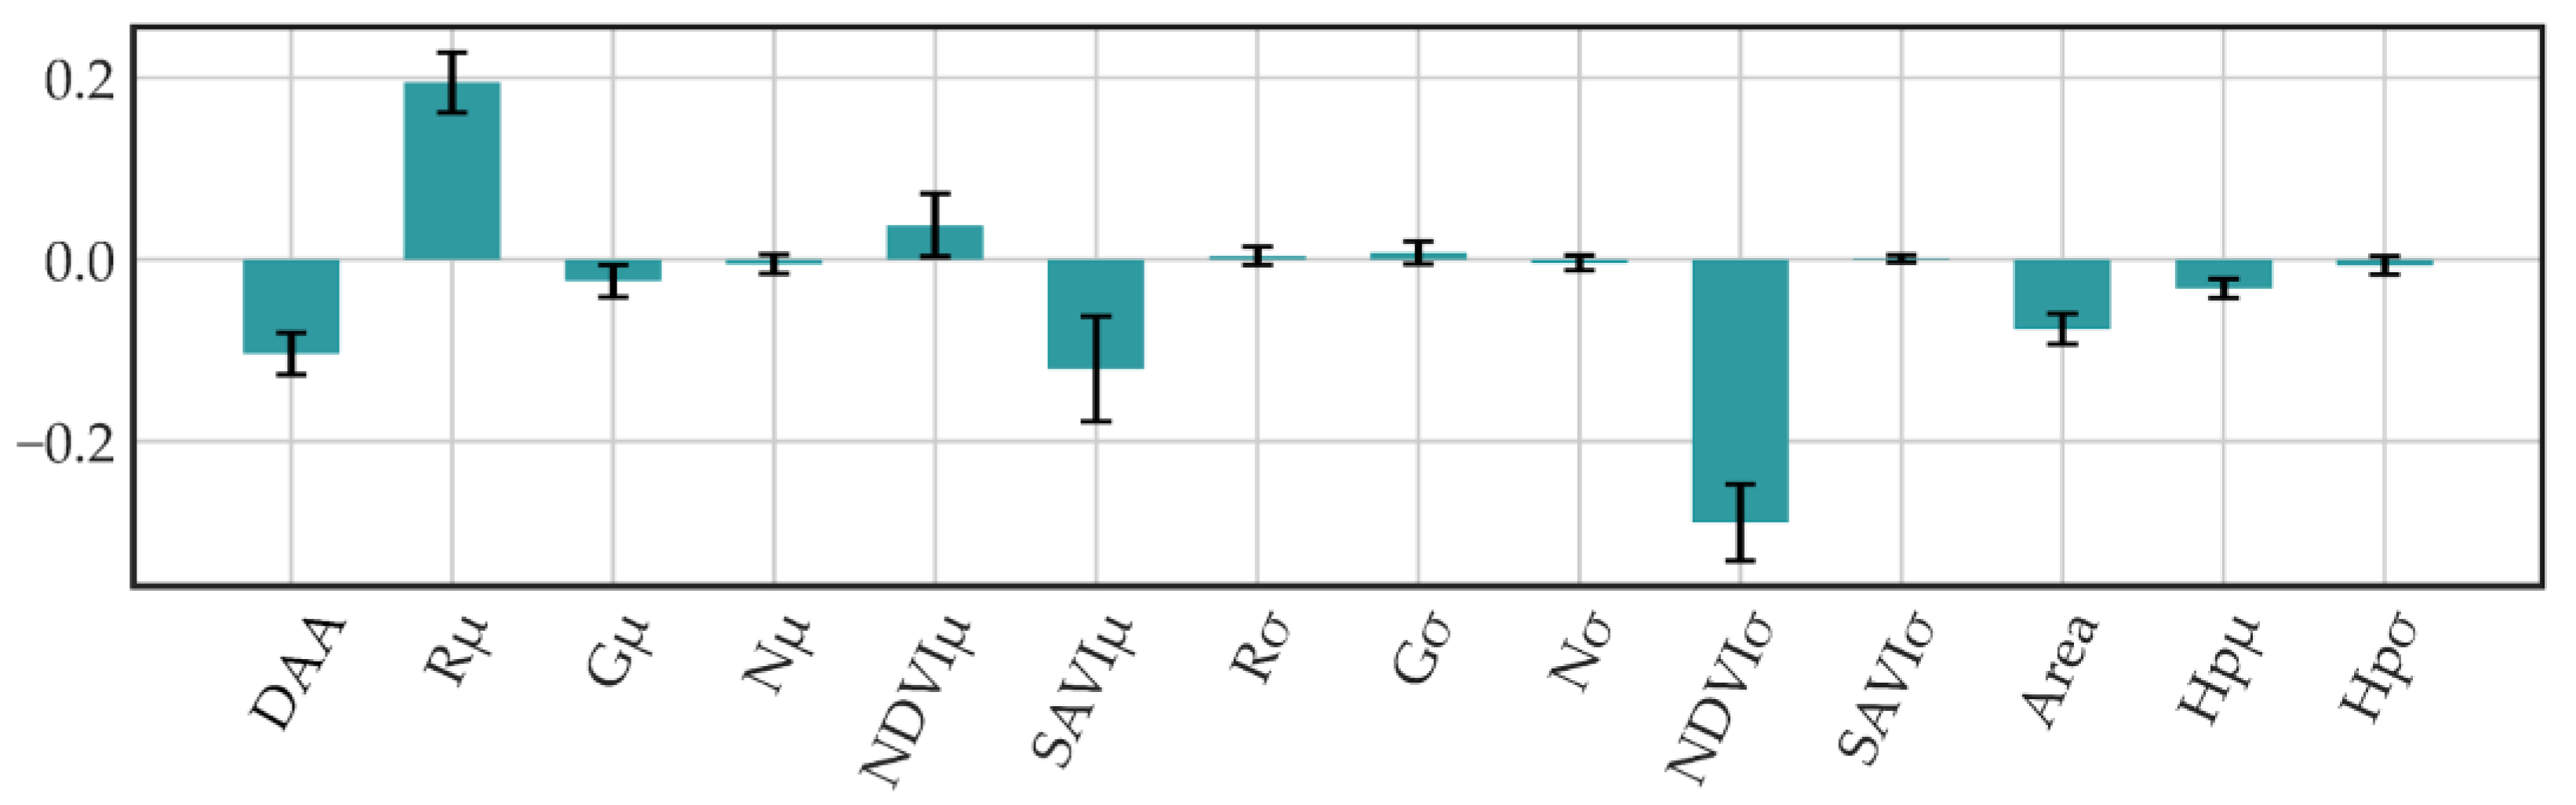
\includegraphics[width=\textwidth]{Images/agronomy-14-00306-g007}
    \caption{Mean values of LASSO $\beta$ coefficients from the 10-fold approach, given for all the predictors. Whisker bars show 1-sigma LASSO $\beta$ estimates.}
    \label{fig:stability}
\end{figure}

\begin{table}[H]
    \centering
    \caption{Mean, standard deviation, and coefficient of variation\textsuperscript{1} values for the coefficients of the LASSO and logistic functions estimated using the 10-fold strategy.}
    \begin{tabular}{lcccc}
    \toprule
    \textbf{Model} & \textbf{Parameter} & \textbf{Mean} & \textbf{Std. dev.} & \textbf{Coef.Var.\textsuperscript{1}} \\
    \midrule
    \multirow{6}{*}{LASSO} & $\beta$ DAA & -0.099 & 0.017 & 0.17 \\
    & $\beta$ R$\mu$ & 0.2 & 0.05 & 0.25 \\
    & $\beta$ SAVI$\mu$ & -0.14 & 0.7 & 0.5 \\
    & $\beta$ NDVI$\sigma$ & -0.28 & 0.04 & 0.14 \\
    & $\beta$ Area & -0.08 & 0.01 & 0.13 \\
    & $\lambda$ & 0.0028 & 0.0013 & 0.46 \\
    \midrule
    \multirow{3}{*}{LF} & $L$ & 94.53 & 1.22 & <0.1 \\
    & $k$ & 0.06 & 0.001 & <0.1 \\
    & $y_0$ & 47.15 & 0.69 & <0.1 \\
    \bottomrule
    \end{tabular}
    \label{tab:LASSO}
    \footnotesize{\textsuperscript{1} Coef.Var. is calculated with the absolute value of the mean.}
\end{table}

nsights into the stability of the model can be gained by observing the coefficient of variation (Coef.Var.) of the most influencing parameters as estimated through the 10-fold strategy. Low values of Coef.Var. across all parameters proved that model stability is ensured. Bands and spectral indices showed the highest values of Coef.Var. This can be related to the significant uncertainty of calibrated reflectance, thus confirming the strict correspondence between measurement errors and the stability of the model (Barbedo et al.
\cite{barbedoDeepLearningApplied2022}).

\subsection{Model Performances}

Descriptive statistics of accuracy metrics were calculated with respect to the K-adjusted models used for predicting PHYGEN. MAE and the adjusted coefficient of determination $Adj R^2$ were calculated for the LASSO model, whereas the coefficient of determination $R^2$ was calculated for the Logistic function trained on LASSO predictions. The adjusted $R^2$ residual degrees of freedom were maintained equal to the number of the LASSO nonzero coefficients
\cite{zouDegreesFreedomLasso2007}. \cref{tab:metrics} shows the results.

\begin{table}[H]
    \centering
    \caption{Fit evaluation metric statistics.}
    \begin{tabular}{lcccc}
    \toprule
    \textbf{Model} & \textbf{} & \textbf{MAE (PHYGEN \%)} & \textbf{$R^2$} & \textbf{Adj $R^2$} \\
    \midrule
    \multirow{2}{*}{LASSO} & Mean & 11.77\% & - & 0.89 \\
    & Std & 0.67\% & - & 0.03 \\
    \midrule
    \multirow{2}{*}{LASSO + LF} & Mean & 10.66\% & 0.9 & - \\
    & Std & 0.83\% & 0.03 & - \\
    \bottomrule
    \end{tabular}
    \label{tab:metrics}
\end{table}

The stacked model predictions ensure a mean absolute error, slightly overcoming the 11\% and having a minimum coefficient of determination
$R_2$ of about 0.9.
Regarding the main goal of this work, it is worth noting that whatever the approach used to obtain an estimate of PHYGEN, its accuracy should be consistent with the one of human evaluation. According to the values reported above, the proposed method is able to provide PHYGEN scores similar to the one from experts. Our estimated accuracy (about 11\%) is close to the reference threshold ordinarily accepted for PPP tests, which is 10\%. Moreover, it presents an 
$R^2$ alue similar to the SOTA model that is trained with a huge amount of data from already tested PPPs due to its CNN architecture
\cite{gomez-zamanilloDamageAssessmentSoybean2023}.
In contrast, MAE values for PHYGEN from our model were about double that obtained from SOTA, which can exploit a huge training set more effectively.
Despite this, we believe that our method is promising and affordable when considering the actual operational conditions for the estimate of PHYGEN for new and untested PPPs, which escapes from the field of application of SOTA, basing deductions on a small training set.

\subsection{Compliance with ANOVA Assumptions}

As previously stated, ANOVA, t-tests, and Z-tests cannot be used with ordinal discrete scale dependent variables 
\cite{stevensTheoryScalesMeasurement1946}.
\cref{fig:ordinal_continuous} shows both the ordinal discrete data used to test the model and the continuous ones from the model. This is a great improvement in the ordinary screening procedures since it enables the possibility of testing group differences through an ANOVA-based approach that a discrete variable excludes.

\begin{figure}[H]
    \centering
    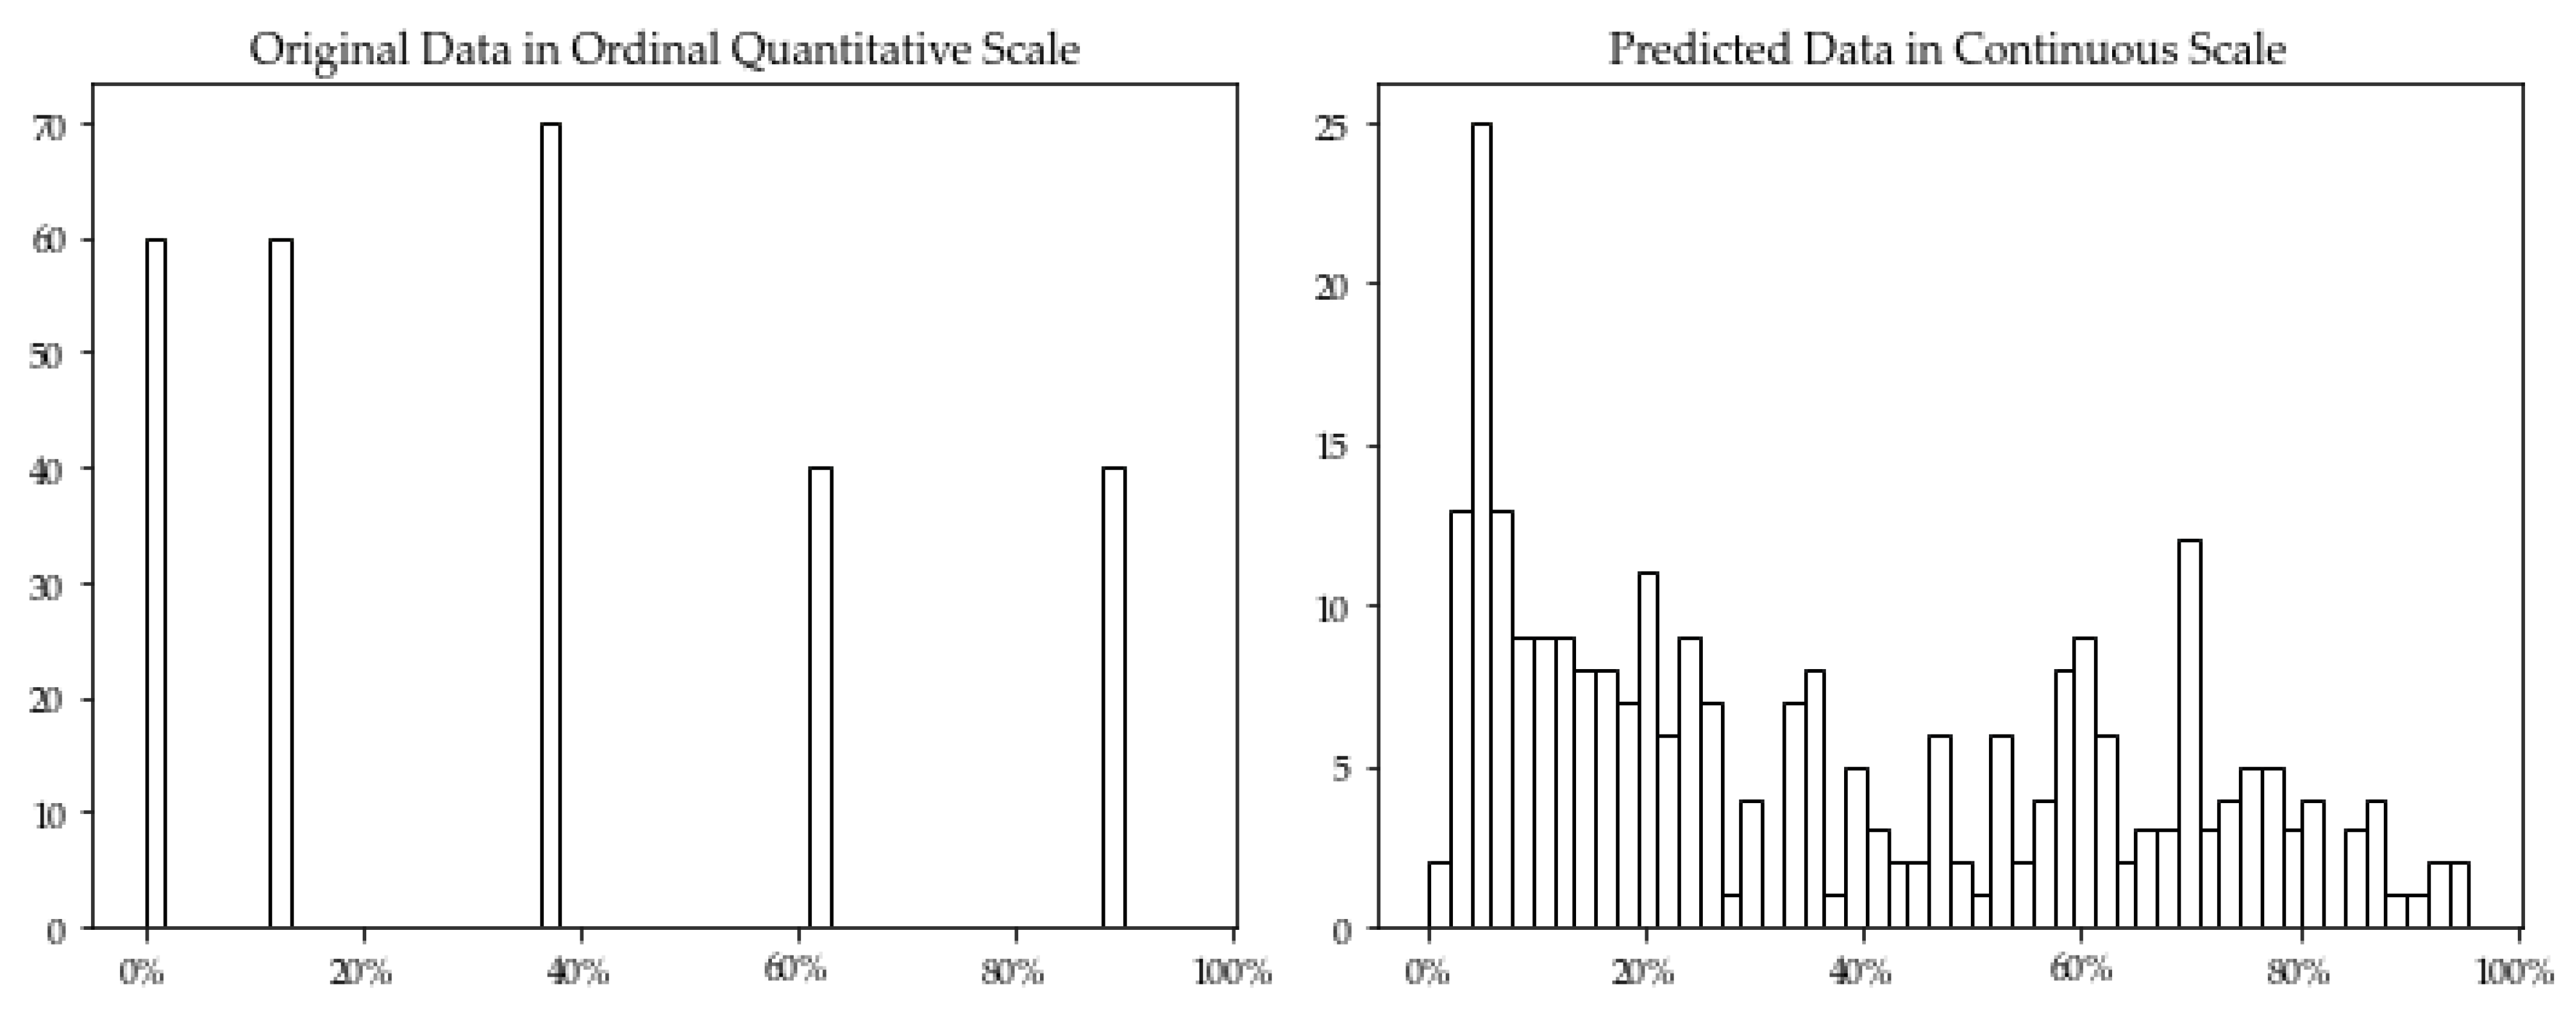
\includegraphics[width=\textwidth]{Images/agronomy-14-00306-g008}
    \caption{Discrete PHYGEN scores from the ordinary human vision-based approach (left). Continuous PHYGEN scores from the model proposed in this work (right).}
    \label{fig:ordinal_continuous}
\end{figure}

\section{Conclusions}

The goal of this study was to test the operability and effectiveness of a controllable simple system based on multispectral digital photogrammetry and AI to support (and improve) current procedures for new PPP screening. This means that the system must be able to generate estimates of ordinarily recognized standard parameters (i.e., PHYGEN) and define the level of phytotoxicity of new PPPs before they enter the market. Basic requirements concern both compliance with accuracy standards and the robustness of the model output.
The proposed method can be made operational if proper Geomatics and AI skills are properly integrated. Geomatic skills are related to proper management of the acquisition system that involves both geometric (image block bundle adjustment) and radiometric-related operations needed to prepare the data that the predictors of the PHYGEN have to be extracted from. Hardware solutions proposed for the system exploit the abovementioned skills with the aim of reducing environmental and sensor-related issues. This makes acquired images more similar, partially overcoming one of the biggest problems recognized for the proper adoption of ML in phytopathometry: image features variability.
A strong constraint introduced by this specific field of study is the lack of a huge training dataset that cannot be reasonably supplied for new PPPs to be screened. In such situations, this type of screening is required.
The system operates in an effectively prepared greenhouse and requires significant infrastructure for the proper movement of the camera and lighting platform.
In this work, we present a simple solution to these requirements. In particular, after suggesting how to pre-process the data from a photogrammetric and radiometric point of view, we found some predictors for the model to be trained that are able to exploit both the geometric and spectral content of acquired data.
The predictors were analyzed and selected. They were used to train an ML algorithm integrating a LASSO and a logistic function to generate continuous estimates of PHYGEN. The robustness of the model was tested by conducting the training with a k-fold strategy and the correspondent statistics analyzed.
The proposed method/system showed stability (robustness), proving to be independent of the training sample. The accuracy of PHYGEN prediction from our model is consistent with the ones from traditional methods. Compared to other AI-based approaches (i.e., SOTA), it showed slightly higher performances in terms of correlation with expert scores applied for new PPPs (our model: $R^2$ = 0.9, SOTA: $R^2$ = 0.89).
In contrast, our model was not able to reach SOTA accuracy in PHYGEN scores prediction (our model: MAE = 10.66\%, SOTA: MAE = 6.74\%). However, it must be noted that SOTA is not intended for predictions concerning new PPPs, and the reference values we reported refer to previously tested PPPs (i.e., providing a huge amount of training data). A surprising capability of the model was to overcome the discrete nature of expert-based scores for PHYGEN. In fact, it is able to generate continuous scores of PHYGEN, even if trained on discrete ones. Their continuous nature provides a high added value since it makes it possible to test differences among groups using ordinary ANOVA-based methods.
However, some improvements are desirable, mostly in relation to a refinement of the hardware of the acquisition platform. A better-performing multispectral camera showing a higher spectral resolution and more rigorous calibration metadata is certainly a first step for future work. The active system providing controlled lighting can also be improved by using light sources that are able to generate a wider spectrum. Camera motion can be improved by using a stepper motor, allowing the possibility to stop the camera during image acquisition, thus avoiding blurring and reducing geometric deformations. Image processing could be also enhanced by strengthening automation in vegetation mask calculation from orthomosaic.
The most significant improvement of the model would be to train a CNN with such a small amount of data. The final activation layer of this CNN should be set to the logistic function proposed in this work. Further studies must test data augmentation techniques and such activation layers with MAE loss to predict PHYGEN in similar setups. Regardless of the solution, we maintain that the explicability of the model, where the physical meaning of predictors and their relationships can be somehow recognized, is an added value for those applications where precise decision making is involved.

\bibliographystyle{plainnat}
\bibliography{SAGEA_DiSAFA}

\end{document}